\documentclass{article}

\usepackage{censor}
\usepackage{geometry}
\usepackage{amsfonts}
\usepackage{amssymb}
\usepackage{amsmath}
\usepackage{fancyhdr}
\usepackage{unicode-math}
\usepackage{titlesec}
\usepackage{siunitx}
\usepackage{setspace}
\usepackage{hyperref}
\usepackage{booktabs}
\usepackage{cleveref}
\usepackage[square, numbers]{natbib}
\usepackage{doi}
\usepackage[numbib]{tocbibind}
\usepackage{minted}
\usepackage{float}
\usepackage{svg}

\bibliographystyle{unsrtnat}
\geometry{left=25mm, right=25mm, top=30mm, bottom=20mm}

\newcommand{\brackets}[1]{\left[\,#1\,\right]}
\newcommand{\paren}[1]{\left( #1 \right)}
\newcommand{\curls}[1]{\left\{#1\right\}}
\newcommand{\verts}[1]{\left\lvert #1 \right\rvert}
\newcommand{\angled}[1]{\left\langle #1 \right\rangle}
\newcommand{\ket}[1]{\left\lvert #1 \right\rangle}
\newcommand{\bra}[1]{\left\langle #1 \right\rvert}

% Sets line number style in minted
\renewcommand{\theFancyVerbLine}{\textcolor[rgb]{0.5,0.5,1.0}{\footnotesize\arabic{FancyVerbLine}}}
% Allows page breaks between math equations
\everymath{\allowdisplaybreaks[2]}
% Fixes space above equations?
\setlength{\abovedisplayskip}{0pt}
% Alternative style section
\titleformat{\section}[block]{\normalfont\itshape}{\thesection}{0.5em}{\titlerule\\[.8ex]\bfseries}

\title{\textbf{Computational and Theoretical Analysis of Structured Light: Quadrupole Interactions in Chiral Molecules} \\ {\small Physics Project \texttt{PHY-6004Y} --- Final Report} }
\date{\textit{27th May 2022}}
\author{100280312}

\begin{document}

\maketitle
\thispagestyle{empty}

\begin{abstract}
	\begin{onehalfspace}
		\noindent This report details the development of computational analysis, including visualization and graphs, of the analytical work in \censor*{14} PhD thesis, which concerns the inclusion of quadrupole molecular moments in the interaction between structured light (a beam possessing orbital angular momentum) and chiral molecules in a paraxial field. The final part of the report generalizes this model for non-paraxial fields.
	\end{onehalfspace}
\end{abstract}

\begin{onehalfspace}
\tableofcontents

\section*{Acknowledgements}
This report is produced as part of the 3\textsuperscript{rd} year ``Physics Project'' module, organized by \censor*{15}.

Many thanks to \censor*{18} and \censor*{18} for supervising me on this report, especially with their expertise on the background knowledge, and thanks to \censor*{10} as well for additional assistance.

\vspace{5mm}

\noindent School of Physics, \censor*{63}.
\end{onehalfspace}

\thispagestyle{empty}
\pagebreak

\begin{onehalfspace}
	\section{Background}\label{sec:background}

	\subsection{Fundamentals of QED}\label{ssec:fundamentals}

	Quantum electrodynamics (QED) is a widely applicable theory in which the interaction between electromagnetic radiation (photons) and matter are quantized. The model of the interaction relies on perturbation theory, applicable in this context as energies from radiation fields produce a relatively small perturbation to the system compared to the intramolecular Coulomb energies\textsuperscript{\citep[pp.~v,~1]{candt}}, around 8 levels of magnitude lower for a continuous laser with an output of \(\SI{e4}{\W.\m^{-2}}\)\textsuperscript{\citep[p.~74]{candt}}. In this section, the necessary background knowledge of number states, the Fermi golden rule, tensors, QED methods, Laguerre-Gaussian beams and optical activity as the basis of the quadrupole model are described.

	\subsubsection{The Hamiltonian}\label{sssec:hamiltonian}

	The time dynamics in quantum mechanics are governed by the time-dependent Schr\"odinger equation,
	\begin{equation}
		i\hbar\frac{\partial}{\partial t}\ket{\symit{Ψ}(t)} = H\ket{\symit{Ψ}(t)}
		\label{eq:schrodinger}
	\end{equation}
	where \(\ket{\symit{Ψ}(t)}\) is the state vector, the representation of the total system.

	Equation (\ref{eq:schrodinger}) is very rarely exactly soluble, and perturbation methods are used to obtain approximate results. In QED, the Hamiltonian is generally defined as follows,
	\begin{equation}
		H = \underbrace{H_\text{mol}+H_\text{rad}}_{H_0}+H_\text{int}
		\label{eq:genhamiltonian}
	\end{equation}
	where \(H_0\) is the unperturbed Hamiltonian, consisting of the molecular and radiation Hamiltonians and \(H_\text{int}\), the interaction Hamiltonian, is treated as the perturbation.

	\subsubsection{Number States}\label{sssec:number}

	The state of the system \(\ket{\symit{Ψ}}\) is typically represented by a wave function. An alternate way, however, is to use number states, also known as ``Fock states'' in an approach known as \textit{second quantization}. They are denoted as
	\begin{equation}
		\ket{\symit{Ψ}} = \ket{n(\symbfit{k},\symit{σ})}
		\label{eq:numberstate}
	\end{equation}
	where \(n\) is the occupation number\textsuperscript{\citep[p.~454]{sakurai}}, the number of particles (assumed to be non-interacting) with wavevector \(\symbfit{k}\) and polarization \(\symit{σ}\).

	At the core of the second quantization formalism are the creation and annihilation operators, which add and remove a particle in a system. They are given respectively by\textsuperscript{\citep[p.~36]{candt}}
	\begin{align}
		a^{\dagger(\symit{σ})}\ket{n(\symbfit{k},\symit{σ})} &= (n+1)^{1/2}\ket{(n+1)(\symbfit{k},\symit{σ})} \qquad n\in\mathbb{N}
		\label{eq:creationoperator}\\
		a^{(\symit{σ})}\ket{n(\symbfit{k},\symit{σ})} &= \begin{cases} n^{1/2}\ket{(n-1)(\symbfit{k},\symit{σ})} &\qquad\quad\! n\in\mathbb{Z}_+ \\ 0 &\qquad\quad\! n=0.\end{cases}
		\label{eq:annihilationoperator}
	\end{align}

	These operators are identical to the ``ladder'' operators (raising and lowering operators) in Dirac's method of finding energies in the quantum harmonic oscillator, which add and remove a quanta of energy\textsuperscript{\citep[p.~136]{qhodirac}}. This is due to the fact that the Hamiltonian for a free electromagnetic field can be written as the sum of the Hamiltonians for a one-dimensional harmonic oscillator\textsuperscript{\citep[p.~35]{candt}} (see future equations (\ref{eq:dmodeexpansion}) and (\ref{eq:bmodeexpansion})), and quantized accordingly depending on which mode is occupied.

	\subsection{Fermi Golden Rule}\label{ssec:fermi}

	The Fermi Golden rule is a measure of the rate of the probability \(P\) of transition between one state and another per unit time, and is defined as\textsuperscript{\citep{fermigoldenrule}}
	\begin{equation}
		\symit{Γ} = \frac{\symup{d}P}{\symup{d}t} = \frac{2\symit{π}}{\hbar}\sum_ξ\verts{M_{fi}(ξ)}^2\symit{ρ}_{\symup{s}}
		\label{eq:fermigolden}
	\end{equation}
	where \(\hbar\) is the reduced Planck constant equal to \(\approx\SI{1.05e-34}{\J\ \s}.\)

	Two factors are of importance in the Fermi Golden rule: first, the matrix element, or the quantum amplitude, which is given by
	\begin{equation}
		M_{fi}(ξ) = \bra{\text{final}}H_\text{int}(ξ)\ket{\text{initial}}
		\label{eq:matrixelement}
	\end{equation}
	for the first order (one photon). Secondly, the density of states, which is defined as the number of levels per unit energy\textsuperscript{\citep[p.~84]{candt}},
	\begin{equation}
		\symit{ρ}_{\symup{s}}=\frac{\symup{d}n}{\symup{d}E}=\frac{1}{\hbar}\frac{\symup{d}n}{\symup{d}\symit{ω}}.
		\label{eq:densityofstates}
	\end{equation}
	where \(\symit{ω}\) is the angular frequency.

	\subsection{The Interaction Hamiltonian and Tensors}\label{ssec:interact}

	The interaction Hamiltonian used in this report is a multipole series in the form known as the Power-Zineau-Woolley Hamiltonian\textsuperscript{\citep{multipolarhamiltonian}},
	\begin{equation}
		H_\text{int} = -\symit{ε}_0^{-1}\iiint\symbfit{p}^\perp(\symbfit{r})\cdot\symbfit{Π}(\symbfit{r})\,\symup{d}^3\symbfit{r} - \iiint\symbfit{m}(\symbfit{r})\cdot\symbfit{b}(\symbfit{r})\,\symup{d}^3\symbfit{r} + \frac{1}{2}\iiint\!\!\!\!\iiint\symbfsf{O}(\symbfit{r},\symbfit{r}')\symbfit{b}(\symbfit{r})\symbfit{b}(\symbfit{r'})\,\symup{d}^3\symbfit{r}\,\symup{d}^3\symbfit{r}'
		\label{eq:pzwhamilunsplit}
	\end{equation}

	which can be split into a sum of specific multipole interactions,
	\begin{align}
		H_\text{int} &= \sum_ξ\brackets{-\symit{ε}_0^{-1}\symit{μ}_i\paren{ξ}d^\perp_i\paren{\symbfit{R}_ξ}-\symit{ε}_0^{-1}Q_{ij}\paren{ξ}\nabla_j d^\perp_i\paren{\symbfit{R}_ξ}-m_i\paren{ξ}b_i\paren{\symbfit{R}_ξ}}\notag\\
		&\phantom{\cdots} + \frac{e^2}{8m}\sum_{ξ,α}\brackets{(\symbfit{q}_{α}(ξ)-\symbfit{R}_{ξ})_i b_j(\symbfit{R}_ξ) ε_{ijk}}^2 + \cdots.
		\label{eq:pzwhamil}
	\end{align}

	From the left, the terms consist of the electric dipole interaction, the electric quadrupole interaction, the magnetic dipole interaction, and the lowest-order diamagnetic coupling interaction.
	
	For background sections up to \S\ref{ssec:opticalactivity}, we will use the electric dipole approximation, which takes only the first term and ignores higher multipole interactions, leaving the Hamiltonian for the interaction coupling as\textsuperscript{\citep[p.~68]{candt}}
	\begin{equation}
		H_\text{int}\paren{ξ}=-\symit{ε}_0^{-1}\symit{μ}_i(ξ)d^\perp_i(\symbfit{R}_ξ)
		\label{eq:electricdipoleapprox}
	\end{equation}
	
	This equation is usually a good approximation as the radiation wavelength is usually larger than the dimensions of the molecules, and so transition probabilities are in large affected by the electric dipole transition moment only. However, this approximation does have caveats, for example, when dealing with shorter wavelengths (like in X-ray spectroscopy) or when dealing with magnetic interactions\textsuperscript{\citep{edaxray}}.

	In equation (\ref{eq:pzwhamil}) we introduce \textit{tensor index notation} (also known as Einstein notation) to denote tensors. Tensors are mathematical objects and can be considered a generalization of scalars (tensor of rank 0) and vectors (tensor of rank 1). A tensor of rank 2 is known as a ``dyad'', contains a magnitude and two directions with each direction spanning over one dimension of space, and can be represented by matrix. Further ranks can be represented by multi-dimensional arrays. In general, a rank \(n\) tensor in a \(m\)-dimensional space will have \(m^n\) components.\textsuperscript{\citep{tensormathworld}}

	A tensor will have indices up to their rank. For example, a vector in 3D space can be written as
	\begin{equation}
		\symbfit{u} = u_1\hat{\symbfit{x}} + u_2\hat{\symbfit{y}} + u_3\hat{\symbfit{z}} = \sum_{n=1}^3 u_n\hat{\symbfit{e}}_n = \begin{bmatrix}u_1 \\ u_2 \\ u_3\end{bmatrix}
		\label{eq:vector}
	\end{equation}
	where \(\{\hat{\symbfit{x}},\hat{\symbfit{y}},\hat{\symbfit{z}}\} \equiv \{\hat{\symbfit{e}}_1,\hat{\symbfit{e}}_2,\hat{\symbfit{e}}_3\}\) are the basis vectors. A rank 2 tensor in 3D space can similarly be constructed as
	\begin{equation}
		\symbf{T} = T_{11}\hat{\symbfit{x}}\hat{\symbfit{x}} + T_{12}\hat{\symbfit{x}}\hat{\symbfit{y}} + T_{13}\hat{\symbfit{x}}\hat{\symbfit{z}} + T_{21}\hat{\symbfit{y}}\hat{\symbfit{x}} + \cdots = \sum_{n=1}^3\sum_{m=1}^3 T_{mn}\hat{\symbfit{e}}_m\hat{\symbfit{e}}_n = \begin{bmatrix}T_{11} & T_{12} & T_{13} \\ T_{21} & T_{22} & T_{23} \\ T_{31} & T_{32} & T_{33}\end{bmatrix}
		\label{eq:rank2tensor}
	\end{equation}
	where \(\{\hat{\symbfit{x}}\hat{\symbfit{x}},\hat{\symbfit{x}}\hat{\symbfit{y}},\cdots\}\) are the unit dyads\textsuperscript{\citep{tensors}}.

	In tensor index notation, summations are implied, and in isolation, a tensor can simply be referred to as \(u_n\) or \(T_{mn}\). By supressing the summation sign, certain calculations are made more convenient. For example, certain vector operations can now be expressed using tensor index notation\textsuperscript{\citep{tensorindex}}. The dot product of two unit vectors can be expressed using the Kronecker delta,
	\begin{equation}
		\hat{\symbfit{e}}_i\cdot \hat{\symbfit{e}}_j = δ_{ij}
		\label{eq:tensorexample1}
	\end{equation}
	where
	\begin{equation}
		δ_{ij}=\begin{cases}1&i=j, \\ 0&\text{otherwise,}\end{cases}
		\label{eq:kronecker}
	\end{equation}
	and so for any two vectors, we have
	\begin{equation}
		\symbfit{u}\cdot\symbfit{v} = (a_i\hat{\symbfit{e}}_i) \cdot (b_j\hat{\symbfit{e}}_j) = a_i b_j \hat{\symbfit{e}}_i\cdot\hat{\symbfit{e}}_j = a_i b_j δ_{ij} = a_i b_i
		\label{eq:tensorexample2}
	\end{equation}
	where in the final step, we performed \textit{Kronecker delta reduction}, which is done by removing \(δ_{ij}\) and setting \(i=j\) in the rest of the equation. This can also be used to reduce expressions such as \(δ_{ij}δ_{jk}δ_{ki} = δ_{ii} = 3\).

	The cross product can be expressed using the Levi-Civita epsilon,
	\begin{equation}
		\hat{\symbfit{e}}_i\times \hat{\symbfit{e}}_j = ε_{ijk}\hat{\symbfit{e}}_k
		\label{eq:tensorexample3}
	\end{equation}
	where
	\begin{equation}
		ε_{ijk}=\begin{cases}1&\curls{i,j,k}=\curls{1,2,3}\text{ or }\curls{2,3,1}\text{ or }\curls{3,1,2}, \\ -1&\curls{i,j,k}=\curls{3,2,1}\text{ or }\curls{2,1,3}\text{ or }\curls{1,3,2}, \\ 0 &\text{otherwise.}\end{cases}
		\label{eq:levicivita}
	\end{equation}
	and for any two vectors,
	\begin{equation}
		\symbfit{u}\times\symbfit{v} = (a_i\hat{\symbfit{e}}_i) \times (b_j\hat{\symbfit{e}}_j) = a_i b_j \hat{\symbfit{e}}_i\times\hat{\symbfit{e}}_j = a_i b_j ε_{ijk} \hat{\symbfit{e}}_k.
		\label{eq:tensorexample4}
	\end{equation}

	\subsection{Rotational Averaging of Tensors}\label{ssec:tensors}

	Certain tensor quantities have an angular dependence, like the electric dipole moment operator \(\symbfit{μ}\) used in the electric dipole approximation (\ref{eq:electricdipoleapprox}) for the interaction coupling. This first-rank tensor depends on the orientation of the molecule, which are in general randomly orientated in gases and liquids. By performing a \textit{rotational average} across each molecule \(ξ\), this dependence can be removed to obtain an end result which is an expression independent on the angle of incident radiation or of the molecule.

	To do this, the components of the tensor are transformed from the laboratory frame, usually denoted with Latin indices \(i,j,k,\dots\) to the molecular frame, usually denoted with Greek indices \(\symit{λ},\symit{μ},ν,\dots\) using an angle matrix denoted \(l_{i_n\symit{λ}_n}\), of which the rotational average can be performed to create a directional cosine \(\langle l_{i_n\symit{λ}_n}\rangle\). For a tensor of rank \(n\), the directional cosine has \(n\) terms \(\langle l_{i_1\symit{λ}_i}\cdots l_{i_n\symit{λ}_n}\rangle\). A non-trigonometric method for calculating the directional cosine, particularly suitable for high \(n\) (and low \(n\) also), described by Andrews and Thirunamachandran\textsuperscript{\citep{rotationalaverage}}, shall be detailed.

	Let \(\langle l_{i_1\symit{λ}_i}\cdots l_{i_n\symit{λ}_n}\rangle\) be denoted as \(I^{(n)}\). \(I^{(n)}\) is rotationally invariant (isotropic), and according to a theorem by Hermann Weyl\textsuperscript{\citep{weyl}}, can be expressed as a linear combination of isotropic tensors. For three-dimensions, the fundamental isotropic unit tensors are the Kronecker delta \(δ_{ij}\), defined in (\ref{eq:kronecker}), and the Levi-Civita epsilon \(ε_{ijk}\), defined in (\ref{eq:levicivita}).
	
	Isotropic tensors of even rank are linear combinations of \(n/2\) Kronecker deltas, and ones of odd ranks are linear combinations of one Levi-Civita epsilon and \((n-3)/2\) deltas. An ``isomer" of a isotropic tensor can be formed by permuting the indices \(i_1, i_2,\dots,i_n\) in a chosen product.

	Using Weyl's theorem from above, it is implied that
	\begin{equation}
		I^{(n)}=\sum_{r,s}m_{rs}^{(n)}f_r^{(n)}g_s^{(n)}
		\label{eq:weylproduct}
	\end{equation}
	where the products \(f^{(n)}\), the tensor in the laboratory frame, and \(g^{(n)}\), the tensor in the molecular frame, are summed over the set of their possible isomers, of which their indices are \(r\) and \(s\). \(m_{rs}^{(n)}\) is therefore a numerical coefficient to be determined. In addition, \(f^{(n)}\) and \(g^{(n)}\) are related for a given isomer \(q\) by
	\begin{equation}
		f_q^{(n)}I^{(n)}=g_q^{(n)},
		\label{eq:labmolproduct}
	\end{equation}
	such that combining equations (\ref{eq:weylproduct}) and (\ref{eq:labmolproduct}) and multiplying through by \(g_t^{(n)}\) gives
	\begin{align}
		f_t^{(n)}f_q^{(n)}&=\sum_{r,s}f_t^{(n)}f_r^{(n)}m_{rs}^{(n)}g_s^{(n)}g_q^{(n)}
		\label{eq:rotavgcombination1}\\
		s_{tq}^{(n)}&=\sum_{r,s}s_{tr}^{(n)}m_{rs}^{(n)}s_{sq}^{(n)}
		\label{eq:rotavgcombination2}
	\end{align}
	as by index-contraction, \(f_u^{(n)}f_v^{(n)}=g_u^{(n)}g_v^{(n)}=s_{uv}^{(n)}\).
	Equation (\ref{eq:rotavgcombination2}) can be expressed in matrix form
	\begin{align}
		S^{(n)}&=S^{(n)}M^{(n)}S^{(n)}
		\label{eq:rotavgmatrix1}\\
		M^{(n)}&=(S^{(n)})^{-1},
		\label{eq:rotavgmatrix2}
	\end{align}
	and it is seen using (\ref{eq:weylproduct}) that \(I^{(n)}\) can be found\textsuperscript{\citep[p.~312]{candt}}.

	Values of \(I^{(n)}\) for \(n=2,\dots, 6\) can be found in \S\ref{ssec:ivalues}.

	\subsection{Single Photon Absorption}\label{ssec:absorption}
	
	Using the information described in \S\ref{sssec:number}, we can write the initial and final states of a molecule absorbing a single photon as
	\begin{align}
		\ket{\text{initial}} &= \ket{n(\symbfit{k},\symit{σ})}\prod_ξ^N\ket{E_o\paren{ξ}}
		\label{eq:onephotoninit}\\
		\ket{\text{final}} &= \ket{(n-1)(\symbfit{k},\symit{σ})}\ket{E_m\paren{ξ}}\prod_{ξ\neq ξ^\prime}^N\ket{E_o\paren{ξ^\prime}}
		\label{eq:onephotonfinal}
	\end{align}
	where the product term represents the molecules (assumed to be non-interacting) in energy level \(E_o\) (before absorption) and \(E_m\) (after absorption).

	However, as any one molecule has an equal probability of absorbing the photon, it is assumed that only molecule \(ξ\) absorbs the photon\textsuperscript{\citep[p.~87]{candt}}, and thus the matrix element is
	\begin{equation}
		M_{fi}(ξ)=\bra{E_m(ξ)}\bra{(n-1)(\symbfit{k},\symit{σ})}-\symit{ε}_0^{-1}\symbfit{μ}(ξ)\cdot\symbfit{d}^\perp(\symbfit{R}_ξ)\ket{n(\symbfit{k},\symit{σ})}\ket{E_o(ξ)},
		\label{eq:onephotonmatel}
	\end{equation}
	where the interaction term of the Hamiltonian is given by the electric dipole approximation previously seen as equation (\ref{eq:electricdipoleapprox}). In addition, we introduce the mode expansion for the field operator \(\symbfit{d}^\perp\), the electric displacement field\textsuperscript{\citep[pp.~36,~68]{candt}}, as
	\begin{equation}
		\symbfit{d}^\perp(\symbfit{r})=\sum_{\symbfit{k},\symit{σ}}\symit{Ω}\{\symbfit{e}^{(\symit{σ})}(\symbfit{k})a^{(\symit{σ})}(\symbfit{k})e^{i\symbfit{k}\cdot\symbfit{r}}-\bar{\symbfit{e}}^{(\symit{σ})}(\symbfit{k})a^{\dagger(\symit{σ})}(\symbfit{k})e^{-i\symbfit{k}\cdot\symbfit{r}}\},
		\label{eq:dmodeexpansion}
	\end{equation}
	where \(\symbfit{e}\) is the polarization vector, \(a^{(\symit{σ})}(\symbfit{k})\), \(a^{\dagger(\symit{σ})}(\symbfit{k})\) are the annihilation and creation operators for the mode \((\symbfit{k},\symit{σ})\), respectively, and the normalization constant \(\symit{Ω}\) is
	\begin{equation}
		\symit{Ω} = i\paren{\frac{\hbar ck\symit{ε}_0}{2V}}^{1/2}
		\label{eq:omeganormalization}
	\end{equation}
	in which \(V\) is the quantization volume.

	We can simplify equation (\ref{eq:onephotonmatel}) as
	\begin{align}
		M_{fi}(ξ) &= \bra{E_m(ξ)}\bra{(n-1)(\symbfit{k},\symit{σ})}-\symit{ε}_0^{-1}\symbfit{μ}(ξ)\cdot\symbfit{d}^\perp(\symbfit{R}_ξ)\ket{n(\symbfit{k},\symit{σ})}\ket{E_o(ξ)} \notag\\
		&=-\symit{ε}_0^{-1}\bra{E_m(ξ)}\symbfit{μ}(ξ)\ket{E_o(ξ)}\cdot\bra{(n-1)(\symbfit{k},\symit{σ})}\symbfit{d}^\perp(\symbfit{R}_ξ)\ket{n(\symbfit{k},\symit{σ})} \notag\\
		&=-\symit{ε}_0^{-1}\symbfit{μ}^{mo}(ξ)\cdot\bra{(n-1)(\symbfit{k},\symit{σ})}\textstyle\sum_{\symbfit{k},\symit{σ}}\symit{Ω}\curls{\symbfit{e}^{(\symit{σ})}(\symbfit{k})a^{(\symit{σ})}(\symbfit{k})e^{i\symbfit{k}\cdot\symbfit{R}_ξ}-\bar{\symbfit{e}}^{(\symit{σ})}(\symbfit{k})a^{\dagger(\symit{σ})}(\symbfit{k})e^{-i\symbfit{k}\cdot\symbfit{R}_ξ}}\ket{n(\symbfit{k},\symit{σ})} \label{eq:onephotonmatelinter1}\\
		&= -\symit{Ω}\symit{ε}_0^{-1}\symbfit{μ}^{mo}(ξ)\cdot\bra{(n-1)(\symbfit{k},\symit{σ})}\symbfit{e}^{(\symit{σ})}(\symbfit{k})a^{(\symit{σ})}(\symbfit{k})e^{i\symbfit{k}\cdot\symbfit{R}_ξ}-\bar{\symbfit{e}}^{(\symit{σ})}(\symbfit{k})a^{\dagger(\symit{σ})}(\symbfit{k})e^{-i\symbfit{k}\cdot\symbfit{R}_ξ}\ket{n(\symbfit{k},\symit{σ})} \label{eq:onephotonmatelinter2}\\
		&= -\symit{Ω}\symit{ε}_0^{-1}\symbfit{μ}^{mo}(ξ)\cdot [\, \bra{(n-1)(\symbfit{k},\symit{σ})}\symbfit{e}^{(\symit{σ})}(\symbfit{k})a^{(\symit{σ})}(\symbfit{k})e^{i\symbfit{k}\cdot\symbfit{R}_ξ}\ket{n(\symbfit{k},\symit{σ})} \notag\\
		&\qquad\qquad\qquad\quad\; -\bra{(n-1)(\symbfit{k},\symit{σ})}\bar{\symbfit{e}}^{(\symit{σ})}(\symbfit{k})a^{\dagger(\symit{σ})}(\symbfit{k})e^{-i\symbfit{k}\cdot\symbfit{R}_ξ}\ket{n(\symbfit{k},\symit{σ})} \,] \notag\\
		&= -\symit{Ω}\symit{ε}_0^{-1}\symbfit{μ}^{mo}(ξ)\cdot [\, \bra{(n-1)(\symbfit{k},\symit{σ})}\symbfit{e}^{(\symit{σ})}(\symbfit{k})e^{i\symbfit{k}\cdot\symbfit{R}_ξ} n^{1/2}\ket{(n-1)(\symbfit{k},\symit{σ})} \notag\\
		&\qquad\qquad\qquad\quad\; -\bra{(n-1)(\symbfit{k},\symit{σ})}\bar{\symbfit{e}}^{(\symit{σ})}(\symbfit{k})e^{-i\symbfit{k}\cdot\symbfit{R}_ξ}(n+1)^{1/2}\ket{(n+1)(\symbfit{k},\symit{σ})} \,] \notag\\
		&= -\symit{Ω}\symit{ε}_0^{-1}\symbfit{μ}^{mo}(ξ)\cdot [\, \bra{(n-1)(\symbfit{k},\symit{σ})}\symbfit{e}^{(\symit{σ})}(\symbfit{k})e^{i\symbfit{k}\cdot\symbfit{R}_ξ} n^{1/2}\ket{(n-1)(\symbfit{k},\symit{σ})} - 0\,] \label{eq:onephotonmatelinter3} \\
		&= -\symit{Ω}\symit{ε}_0^{-1}n^{1/2} \symbfit{μ}^{mo}(ξ)\cdot \symbfit{e}^{(\symit{σ})}(\symbfit{k})e^{i\symbfit{k}\cdot\symbfit{R}_ξ}
		\label{eq:onephotonmatelfinal}
	\end{align}

	where in (\ref{eq:onephotonmatelinter1}) we write \(\symbfit{μ}^{mo}(ξ)\) as the electric dipole moment for the transition \(m\leftarrow o\), in (\ref{eq:onephotonmatelinter2}) the sum is taken over the singular mode \((\symbfit{k},\symit{σ})\), and in (\ref{eq:onephotonmatelinter3}) the second term reduces to zero due to the orthonormality of the number state kets \(\angled{n' \mid n} = δ_{n'n}\).

	After (\ref{eq:onephotonmatelfinal}) the transition rate given by the Fermi golden rule (\ref{eq:fermigolden}) is
	\begin{align}
		\symit{Γ}&=\frac{2\symit{π}}{\hbar}\symit{ρ}_{\symup{s}}\paren{\frac{\symit{Ω}^2n}{\symit{ε}_0^2}}\sum_ξ|\symbfit{μ}^{mo}(ξ)\cdot\symbfit{e}^{(\symit{σ})}(\symbfit{k})e^{i\symbfit{k}\cdot\symbfit{R}_ξ}|^2 = \frac{2\symit{π}}{\hbar}\symit{ρ}_{\symup{s}}\paren{\frac{\symit{Ω}^2n}{\symit{ε}_0^2}}\sum_ξ|\symbfit{μ}^{mo}(ξ)\cdot\symbfit{e}^{(\symit{σ})}(\symbfit{k})|^2\notag\\
		&=\frac{2\symit{π}}{\hbar}\symit{ρ}_{\symup{s}}\paren{\frac{\symit{Ω}^2n}{\symit{ε}_0^2}}e_i^{(\symit{σ})}(\symbfit{k})\bar{e}_j^{(\symit{σ})}(\symbfit{k})\sum_ξ \symit{μ}_i^{mo}(ξ)\bar{\symit{μ}}_j^{mo}(ξ).
		\label{eq:finally}
	\end{align}

	The term \(\symit{μ}_i^{mo}(ξ)\bar{\symit{μ}}_j^{mo}(ξ)\), a tensor of rank 2, in equation (\ref{eq:finally}) can be rotationally averaged using the formula in \S\ref{ssec:ivalues} to obtain\textsuperscript{\citep[p.~88]{candt}}
	\begin{align}
		\angled{\symit{Γ}\,}&=\frac{2\symit{π}}{\hbar}\symit{ρ}_{\symup{s}}\paren{\frac{\symit{Ω}^2n}{\symit{ε}_0^2}}e_i^{(\symit{σ})}(\symbfit{k})\bar{e}_j^{(\symit{σ})}(\symbfit{k})\sum_ξ\frac{1}{3}δ_{ij}δ_{\symit{λ}\symit{μ}}\symit{μ}_{\symit{λ}}^{mo}\paren{ξ}\bar{\symit{μ}}_{\symit{μ}}^{mo}\paren{ξ}\notag\\
		&=\frac{2\symit{π}}{\hbar}\frac{N}{3}\symit{ρ}_{\symup{s}}\paren{\frac{\symit{Ω}^2n}{\symit{ε}_0^2}}e_i^{(\symit{σ})}(\symbfit{k})\bar{e}_i^{(\symit{σ})}(\symbfit{k})\symit{μ}_{\symit{λ}}^{mo}\bar{\symit{μ}}_{\symit{λ}}^{mo}\notag\\
		&=\frac{2\symit{π}}{\hbar}\frac{N}{3}\symit{ρ}_{\symup{s}}\paren{\frac{\symit{Ω}^2n}{\symit{ε}_0^2}}\verts{\symbfit{μ}^{mo}}^2
		\label{eq:finallyrotavg}
	\end{align}
	where the summation over \(ξ\) is replaced with \(N\), the number of absorbers.

	\subsection{Two Photon Absorption}\label{ssec:twophoton}

	In order to continue with two photon absorption we must make an adjustment to the matrix element formula (\ref{eq:matrixelement}) to two photons. When more than one photon is absorbed, there are a number of intermediate states \(\ket{I}\) between the initial state \(\ket{i}\) and final state \(\ket{f}\). By performing a second-order pertubative analysis\textsuperscript{\citep[p.~109]{candt}}\textsuperscript{\citep[p.~241]{brennan}}, the matrix element is found as
	\begin{equation}
		M_{fi} = \sum_{I} \frac{\bra{f}H_\text{int}\ket{I}\bra{I}H_\text{int}\ket{i}}{E_I - E_i}.
		\label{eq:matrixelement2}
	\end{equation}

	In general, the matrix element can be written as
	\begin{equation}
		M_{fi} = \bra{f}H_\text{int}\ket{i} + \sum_{I} \frac{\bra{f}H_\text{int}\ket{I}\bra{I}H_\text{int}\ket{i}}{E_I - E_i} + \sum_{I, I\!I} \frac{\bra{f}H_\text{int}\ket{I\!I}\bra{I\!I}H_\text{int}\ket{I}\bra{I}H_\text{int}\ket{i}}{(E_I - E_i)(E_{I\!I} - E_i)} + \cdots
		\label{eq:genmatrixelement}
	\end{equation}
	but in two-photon absorption, there is only one intermediate state, and higher intermediate states are ignored; the first term cancels to 0 as the occupation numbers differ by 2, and so a transition cannot be made according to the selection rules. The energy from the initial to the intermediate state \(E_{iI}\) is calculated as \(E_r + (n-1)\hbar\symit{ω} - E_o - n\hbar\symit{ω} = E_{ro} - \hbar\symit{ω}\). After subsituting the initial and final states, and assuming that both photons come from the same beam, we obtain

	\begin{align}
		M_{fi} = \sum_{r}\frac{1}{E_{or}-\hbar \symit{ω}} \Big[&\bra{E_m}\bra{(n-2)(\symbfit{k},\symit{σ})}-\symit{ε}_0^{-1}\symbfit{μ}(ξ)\cdot\symbfit{d}^\perp(\symbfit{R}_ξ)\ket{(n-1)(\symbfit{k},\symit{σ})}\ket{E_r}\notag\\
		\times &\bra{E_r}\bra{(n-1)(\symbfit{k},\symit{σ})}-\symit{ε}_0^{-1}\symbfit{μ}(ξ)\cdot\symbfit{d}^\perp(\symbfit{R}_ξ)\ket{n(\symbfit{k},\symit{σ})}\ket{E_o}\Big]
		\label{eq:twophotonmatrixelement}
	\end{align}
	and can be simplified in a similar process as in \S\ref{ssec:absorption} as
	\begin{align}
		M_{fi} &= \frac{1}{\symit{ε}_0^2}\sum_{r}\frac{\bra{E_m}\symbfit{μ}(ξ)\ket{E_r} \bra{E_r}\symbfit{μ}(ξ)\ket{E_o} }{E_{or}-\hbar \symit{ω}} \cdot \Big[\bra{(n-2)(\symbfit{k},\symit{σ})}\symbfit{d}^\perp(\symbfit{R}_ξ)\ket{(n-1)(\symbfit{k},\symit{σ})}\notag\\
		&\qquad\qquad\qquad\qquad\qquad\qquad\qquad\qquad\qquad\times \bra{(n-1)(\symbfit{k},\symit{σ})}\symbfit{d}^\perp(\symbfit{R}_ξ)\ket{n(\symbfit{k},\symit{σ})}\Big] \notag\\
		&=\frac{\symit{Ω}^2}{\symit{ε}_0^2}\sum_r\paren{\frac{\symit{μ}_i^{mr}(ξ)\symit{μ}_j^{ro}(ξ)}{E_{or}-\hbar \symit{ω}}}\cdot \brackets{\paren{(n-1)^{1/2}\symbfit{e}^{(\symit{σ})}(\symbfit{k})e^{i\symbfit{k}\cdot\symbfit{R}_ξ}}\paren{n^{1/2}\symbfit{e}^{(\symit{σ})}(\symbfit{k})e^{i\symbfit{k}\cdot\symbfit{R}_ξ}}} \notag\\
		&=\frac{\symit{Ω}^2}{\symit{ε}_0^2}\sum_r\paren{\frac{\symit{μ}_i^{mr}(ξ)\symit{μ}_j^{ro}(ξ)}{E_{or}-\hbar \symit{ω}}}\cdot \curls{n(n-1)}^{1/2}e_i^{(\symit{σ})}(\symbfit{k})e_j^{(\symit{σ})}(\symbfit{k})e^{2i\symbfit{k}\cdot\symbfit{R}_ξ}.
	\end{align}

	Since the term \(e_i^{(\symit{σ})}(\symbfit{k})e_j^{(\symit{σ})}(\symbfit{k})\) are symmetric in \(i,j\), contraction with the \(r\)-summed term will leave only the \(i,j\)-symmetric part, and we can write

	\begin{align}
		M_{fi}&=\frac{\symit{Ω}^2}{2\symit{ε}_0^2}\sum_r\paren{\frac{\symit{μ}_i^{mr}(ξ)\symit{μ}_j^{ro}(ξ)}{E_{or}-\hbar \symit{ω}} + \frac{\symit{μ}_j^{mr}(ξ)\symit{μ}_i^{ro}(ξ)}{E_{or}-\hbar \symit{ω}}}\cdot \curls{n(n-1)}^{1/2}e_i^{(\symit{σ})}(\symbfit{k})e_j^{(\symit{σ})}(\symbfit{k})e^{2i\symbfit{k}\cdot\symbfit{R}_ξ} \notag\\
		&=\frac{\symit{Ω}^2}{2\symit{ε}_0^2} \symbfup{α}^{mo} \curls{n(n-1)}^{1/2}e_i^{(\symit{σ})}(\symbfit{k})e_j^{(\symit{σ})}(\symbfit{k})e^{2i\symbfit{k}\cdot\symbfit{R}_ξ}
		\label{eq:finally2}
	\end{align}
	where in (\ref{eq:finally2}) we introduced a rank 2 tensor \(\symbfup{α}^{mo}\) which will need to be rotationally averaged after we find the transition rate as
	\begin{equation}
		\angled{\symit{Γ}\,} = \frac{2\symit{π}}{\hbar}N\symit{ρ}_{\symup{s}}\frac{\symit{Ω}^4}{4\symit{ε}_0^4} n(n-1)e_i^{(\symit{σ})}(\symbfit{k})e_j^{(\symit{σ})}(\symbfit{k})\bar{e}_k^{(\symit{σ})}(\symbfit{k})\bar{e}_l^{(\symit{σ})}(\symbfit{k})\angled{\symup{α}^{mo}_{ij}\bar{\symup{α}}^{mo}_{kl}}.
	\end{equation}
	
	Using the formula in \S\ref{ssec:ivalues} again,
	\begin{align}
		\angled{\symup{α}_{ij}^{mo}\bar{\symup{α}}_{kl}^{mo}}=\frac{1}{30}&[\,δ_{ij}δ_{kl}(4δ_{\symit{λ}\symit{μ}}δ_{\symit{ν}\symit{π}}-δ_{\symit{λ}\symit{ν}}δ_{\symit{μ}\symit{π}}-δ_{\symit{λ}\symit{π}}δ_{\symit{μ}\symit{ν}}) \notag\\
		+&\,\,δ_{ik}δ_{jl}(-δ_{\symit{λ}\symit{μ}}δ_{\symit{ν}\symit{π}}+4δ_{\symit{λ}\symit{ν}}δ_{\symit{μ}\symit{π}}-δ_{\symit{λ}\symit{π}}δ_{\symit{μ}\symit{ν}}) \notag\\
		+&\,\,δ_{il}δ_{jk}(-δ_{\symit{λ}\symit{μ}}δ_{\symit{ν}\symit{π}}-δ_{\symit{λ}\symit{ν}}δ_{\symit{μ}\symit{π}}+4δ_{\symit{λ}\symit{π}}δ_{\symit{μ}\symit{ν}})\,]\symup{α}_{\symit{λ}\symit{μ}}^{mo}\bar{\symup{α}}_{\symit{ν}\symit{π}}^{mo}
	\end{align}
	in which the Greek indices can be contracted and the \(\symit{λ},\symit{μ}\)-symmetric property of \(\symup{α}_{\symit{λ}\symit{μ}}^{mo}\) be exploited to obtain
	\begin{equation}
		\angled{\symup{α}_{ij}^{mo}\bar{\symup{α}}_{kl}^{mo}}=\frac{1}{30} \brackets{ \delta_{ij}\delta_{kl}\{4\symup{α}_{\symit{λ}\symit{λ}}^{mo}\bar{\symup{α}}_{\symit{μ}\symit{μ}}^{mo}-2\symup{α}_{\symit{λ}\symit{μ}}^{mo}\bar{\symup{α}}_{\symit{λ}\symit{μ}}^{mo}\} - (\delta_{ik}\delta_{jl}+\delta_{il}\delta_{jk})\{\symup{α}_{\symit{λ}\symit{λ}}^{mo}\bar{\symup{α}}_{\symit{μ}\symit{μ}}^{mo}-3\symup{α}_{\symit{λ}\symit{μ}}^{mo}\bar{\symup{α}}_{\symit{λ}\symit{μ}}^{mo}\} }.
		\label{eq:finally2rotavgpre}
	\end{equation}

	Combining (\ref{eq:finally2rotavgpre}) with the polarization tensors (whose \(\symit{σ}\) and \(\symbfit{k}\) labels are suppressed for brevity),
	\begin{equation}
		e_ie_j\bar{e}_k\bar{e}_l \angled{\symup{α}_{ij}^{mo}\bar{\symup{α}}_{kl}^{mo}} = \frac{1}{15} \brackets{ (2e_ie_j\bar{e}_k\bar{e}_l-1)\symup{α}_{\symit{λ}\symit{λ}}^{mo}\bar{\symup{α}}_{\symit{μ}\symit{μ}}^{mo} - (e_ie_j\bar{e}_k\bar{e}_l-3)\symup{α}_{\symit{λ}\symit{μ}}^{mo}\bar{\symup{α}}_{\symit{λ}\symit{μ}}^{mo}}
	\end{equation}
	such that the absorption rate can be found to be\textsuperscript{\citep[p.~114]{candt}}
	\begin{equation}
		\angled{\symit{Γ}\,} = \frac{\symit{π}}{30\hbar}\frac{\symit{Ω}^4}{\symit{ε}_0^4}N\symit{ρ}_{\symup{s}} n(n-1)\brackets{ (2e_ie_j\bar{e}_k\bar{e}_l-1)\symup{α}_{\symit{λ}\symit{λ}}^{mo}\bar{\symup{α}}_{\symit{μ}\symit{μ}}^{mo} - (e_ie_j\bar{e}_k\bar{e}_l-3)\symup{α}_{\symit{λ}\symit{μ}}^{mo}\bar{\symup{α}}_{\symit{λ}\symit{μ}}^{mo}}.
		\label{eq:finally2rotavg}
	\end{equation}

	\subsection{Laguerre-Gaussian Beams}\label{ssec:beams}

	When light is emitted from a laser, it will have a beam profile, determined by the design and fabrication of the laser. Most ideal laser beams will have a Gaussian intensity profile, where the irradiance of the beam away from its centre point is proportional to \(e^{-r^2}\), as much of the energy is focused onto the intended, most concentrated spot.\textsuperscript{\citep{gaussianbeam}}

	Laguerre-Gaussian beams are a mathematic representation of a Gaussian beam which occur as a modal decomposition of the paraxial scalar Helmholtz equation, a specific representation of the wave equation. In addition, L-G beams have cylindrical symmetry and the electric displacement and magnetic field mode expansions for the L-G beam express a dependence on \(\ell\), which determines the twist structure of the orbital angular momentum of the beam, which are used as the basis of structured light\textsuperscript{\citep{lgbeam}}.

	In cylindrical coordinates, the paraxial scalar Helmholtz equation is
	\begin{equation}
		\paren{\frac{1}{\symit{ρ}}\frac{\partial}{\partial \symit{ρ}} + \frac{\partial^2}{\partial^2 \symit{ρ}} + \frac{1}{\symit{ρ}^2}\frac{\partial^2}{\partial \symit{φ}^2} + 2ik\frac{\partial}{\partial z}}u\paren{\symit{ρ},\symit{φ},z}=0.
		\label{eq:helmholtz}
	\end{equation}

	The normalized amplitude of the Laguerre-Gaussian beam, a solution to \(u\paren{\symit{ρ},\symit{φ},z}\) above, is:
	\begin{equation}
		u_{\ell,p}^\text{LG}\paren{\symit{ρ},\symit{φ},z}=\frac{C_p^{\verts{\ell}}}{w(z)}\paren{\frac{\sqrt{2}\symit{ρ}}{w(z)}}^{\verts{\ell}}\!\!\!L_p^{\verts{\ell}}\paren{\frac{2\symit{ρ}^2}{w^2(z)}}\exp\paren{-\frac{\symit{ρ}^2}{w^2(z)}-ik\frac{k\symit{ρ}^2z}{2(z^2+z_{\symup{R}}^2)}-i\ell \symit{φ}+i(2p+\ell+1)\arctan\paren{\frac{z}{z_{\symup{R}}}}}
		\label{eq:lgbeam}
	\end{equation}
	where \(p\) is the radial index, \(\ell\) is the topological charge, \(w(z)\) is the beam waist, the radius of the beam at \(z\), given by
	\begin{equation}
		w(z) = w(0)\paren{1+\frac{z^2}{z_{\symup{R}}^2}}^{1/2},
	\end{equation}
	\(z_{\symup{R}}\) is the Rayleigh range (figure \ref{fig:rayleighrange}), a measure of the beam's focal length, \(L_p^{\verts{\ell}}\) is the generalized Laguerre polynomial of order \(p\), which is given by
	\begin{equation}
		L_p^{\ell}\paren{x} = \sum_{n=0}^p \paren{-1}^n\begin{pmatrix}p+\ell \\ p-n\end{pmatrix}\frac{x^n}{n!},
		\label{eq:genlaguerre}
	\end{equation}
	and the normalization constant \(C_p^{\verts{\ell}}\) is given by
	\begin{equation}
		C_p^{\verts{\ell}} = \paren{2^{\verts{\ell}+1}\frac{p!}{\symit{π}\paren{p+\verts{\ell}}!}}^{1/2}.
		\label{eq:normalizationconstant}
	\end{equation}

	\begin{figure}[h]
		\centering
			\includesvg[width=0.6\textwidth]{svg/gaussian_beam_waist}
		\caption{The Rayleigh range \(z_{\symup{R}}\), which can be defined as the distance from \(\sqrt{2}\) times the central beam width. Adapted from Rodolfo Hermans, under GFDL (GNU Free Distribution License).}
		\label{fig:rayleighrange}
	\end{figure}

	In most circumstances the Rayleigh range for L-G beams is around several metres, and in considering beam interactions with particles we can approximate equation (\ref{eq:lgbeam}) by considering it in the long Rayleigh range \(z_{\symup{R}}\gg z\) (i.e.~the beam width is constant). By rewriting
	\begin{align}
		w\paren{z} &\approx w_0 := w(0) \\
		\frac{1}{z^2+z_{\symup{R}}^2} &\approx 0 \\
		\arctan\paren{\frac{z}{z_{\symup{R}}}} &\approx 0
	\end{align}
	and defining the \textit{radial distribution function} as
	\begin{equation}
		f_{\ell, p}\paren{\symit{ρ}} = \frac{C_p^{\verts{\ell}}}{w_0}\paren{\frac{\sqrt{2}\symit{ρ}}{w_0}}^{\verts{\ell}}e^{-\symit{ρ}^2/w_0^2}L_p^{\verts{\ell}}\paren{\frac{2\symit{ρ}^2}{w_0^2}},
		\label{eq:rdfunction}
	\end{equation}
	the amplitude of the Laguerre-Gaussian beam can then be expressed, without \(z\) dependence, as 
	\begin{equation}
		u_{\ell,p}^\text{LG}\paren{\symit{ρ},\symit{φ}}\approx f_{\ell, p}\paren{\symit{ρ}}e^{-i\ell\symit{φ}}.
		\label{eq:rdflgapprox}
	\end{equation}

	\subsection{Optical Activity}\label{ssec:opticalactivity}

	\begin{figure}[h]
		\centering
		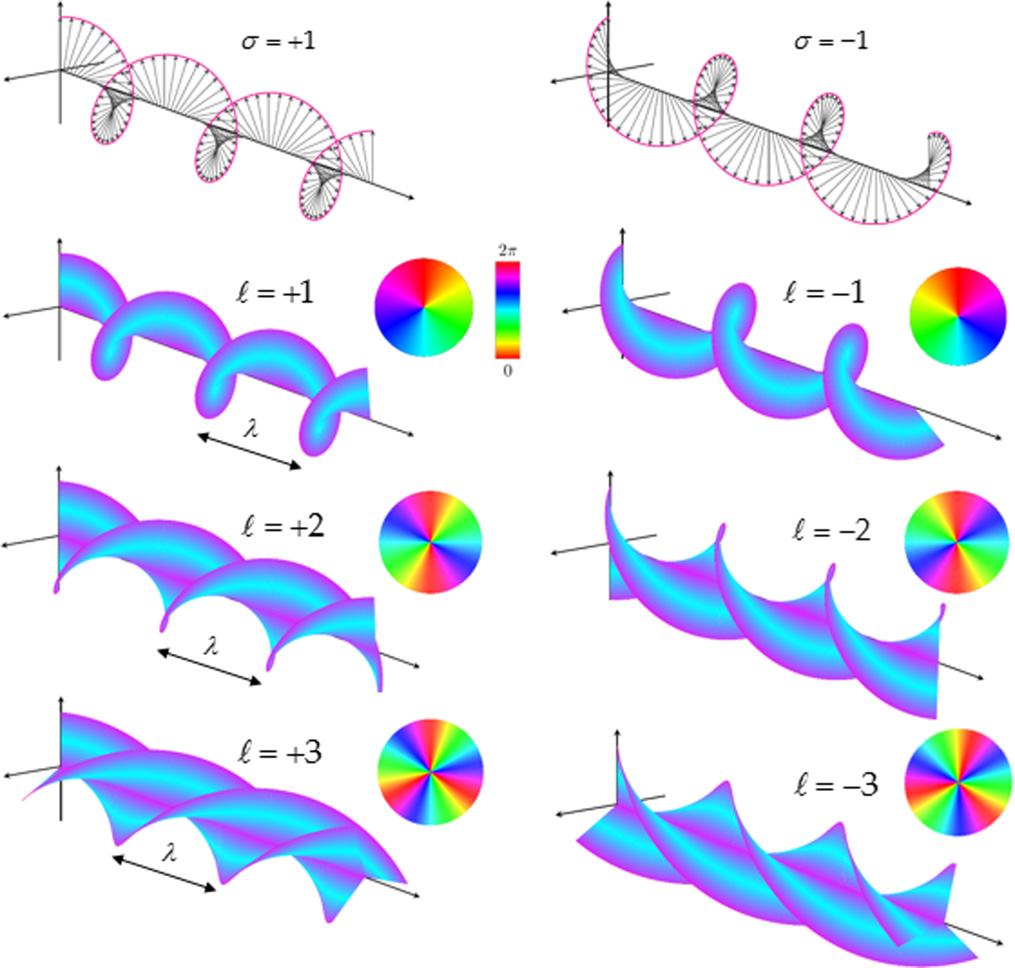
\includegraphics[width=0.8\textwidth]{chirality_of_light.jpg}
		\caption{The visualization of the chirality of light. \textbf{T{\scriptsize OP:}} Electric field vectors for beams with left- and right-circular polarizations possessing spin angular momentum. \textbf{B{\scriptsize OTTOM:}} Wavefronts of beams with various topological charges \(\ell\), which are generally considered the source of the beam's orbital angular momentum\textsuperscript{\citep{twistedlightoam}}.}
	\end{figure}

	Optical activity is the difference in the responses of chiral, or optically active molecules, when exposed to light radiation with angular momentum. Chiral molecules are molecules that cannot be superposed onto its mirror image by means of rotation or translation\textsuperscript{\citep{chirality}}, and belong to point groups with no improper axis of rotation \(C_n, D_n, T, O, I\)\textsuperscript{\citep[p.~183]{candt}}. The angular momentum of light can manifest itself in two different ways: the first, \textit{spin angular momentum}, quantized by \(\symit{σ}\hbar\) per photon and appears in circularly polarized beams; and the second, \textit{orbital angular momentum}, quantized by \(\ell\hbar\) per photon in beams with a twisting wavefront\textsuperscript{\citep{twistedlightoam}}, and are such called ``structured light'' or ``optical vortices''\textsuperscript{\citep{vortexdichroism}}.
	
	The chiroptical properties are examined in this subsection are circular dichroism, which is the differential absorption of circularly polarized light, and then by extension, circular vortex dichroism, the differential absorption of circularly polarized light with optical vortices. Vortex dichroism can also occur in plane polarized beams\textsuperscript{\citep{vdplanepolarized}}, as is discussed later in \S\ref{sec:Discussion}.

	\subsubsection{Circular Dichroism}\label{sssec:dichroism}

	Circular dichroism is the phenomenon under which left-circularly polarized and right-circularly polarized light are absorbed at a different rate by chiral molecules. A similar method to what is shown in \S\ref{ssec:absorption} can be used, but the electric dipole approximation for the interaction term is insufficient in this context as circular dichroism arises from an interference of electric dipole and magnetic dipole moments\textsuperscript{\citep[pp.~99,~185]{candt}}, and therefore it is necessary for the first magentic dipole term in the multipolar Hamiltonian to be included:
	\begin{equation}
		H_\text{int} = -\symit{ε}_0^{-1}\symit{μ}_i\paren{ξ}d^\perp_i\paren{\symbfit{R}_ξ} - m_i\paren{ξ}b_i\paren{\symbfit{R}_ξ}.
		\label{eq:circulardichroismhint}
	\end{equation}

	We can now proceed with the substitution \(\symit{σ}=\symup{L}(+1)/\symup{R}(-1)\), where L and R stand for left- and right-circularly polarized, respectively. Our matrix element is
	\begin{equation}
		M_{fi}^{\symup{L}/\symup{R}} = -\symit{ε_0}^{-1}\symbfit{μ}^{mo}(ξ)\cdot\bra{(n-1)(\symbfit{k},\symup{L}/\symup{R})}\symbfit{d}^\perp(\symbfit{R}_ξ)\ket{n(\symbfit{k},\symup{L}/\symup{R})} - \symbfit{m}^{mo}(ξ)\cdot\bra{(n-1)(\symbfit{k},\symup{L}/\symup{R})}\symbfit{b}(\symbfit{R}_ξ)\ket{n(\symbfit{k},\symup{L}/\symup{R})}.
		\label{eq:cdmatel1}
	\end{equation}
	
	The mode expansion for the magnetic field \(\symbfit{b}\) is\textsuperscript{\citep[p.~36]{candt}}
	\begin{equation}
		\symbfit{b}(\symbfit{r}) = \sum_{\symbfit{k},\symit{σ}}\frac{\symit{Ω}}{c\symit{ε}_0}\{\symbfit{b}^{(\symit{σ})}(\symbfit{k})a^{(\symit{σ})}(\symbfit{k})\mathrm{e}^{i\symbfit{k}\cdot\symbfit{r}}-\bar{\symbfit{b}}^{(\symit{σ})}(\symbfit{k})a^{\dagger(\symit{σ})}(\symbfit{k})\mathrm{e}^{-i\symbfit{k}\cdot\symbfit{r}}\}.
		\label{eq:bmodeexpansion}
	\end{equation}
	where \(\symbfit{b}^{(\symit{σ})}(\symbfit{k})\) is the polarization tensor in the direction of the magnetic field, perpendicular to the electric field per \(\symbfit{b} = \hat{\symbfit{z}}\times\symbfit{e}\) such that
	\begin{equation}
		\symbfit{b}^{(\symup{L}/\symup{R})}(\symbfit{k}) = \mp i\symbfit{e}^{(\symup{L}/\symup{R})}(\symbfit{k}).
	\end{equation}

	Continuing from (\ref{eq:cdmatel1}), and for convenience, dropping photon mode labels for occupation numbers (which will be done to the end)
	\begin{align}
		M_{fi}^{\symup{L}/\symup{R}} &= -\frac{\symit{Ω}}{\symit{ε}_0}n^{1/2} \symbfit{μ}^{mo}(ξ)\cdot \symbfit{e}^{(\symup{L}/\symup{R})}(\symbfit{k})e^{i\symbfit{k}\cdot\symbfit{R}_ξ} - \frac{\symit{Ω}}{c\symit{ε}_0}\symbfit{m}^{mo}(ξ)\cdot [\,\bra{n-1}\symbfit{b}^{(\symup{L}/\symup{R})}(\symbfit{k})a^{(\symup{L}/\symup{R})}(\symbfit{k})\mathrm{e}^{i\symbfit{k}\cdot\symbfit{R_ξ}}\ket{n}\notag\\
		&\qquad\qquad\qquad\qquad\qquad\qquad\qquad\qquad\qquad\qquad\quad\;\, -\bra{n-1}\bar{\symbfit{b}}^{(\symup{L}/\symup{R})}(\symbfit{k})a^{\dagger(\symup{L}/\symup{R})}(\symbfit{k})\mathrm{e}^{-i\symbfit{k}\cdot\symbfit{R_ξ}}\ket{n} \,] \notag\\
		&= -\frac{\symit{Ω}}{\symit{ε}_0}n^{1/2} \symbfit{μ}^{mo}(ξ)\cdot \symbfit{e}^{(\symup{L}/\symup{R})}(\symbfit{k})e^{i\symbfit{k}\cdot\symbfit{R}_ξ} - \frac{\symit{Ω}}{c\symit{ε}_0}n^{1/2}\symbfit{m}^{mo}(ξ)\cdot\symbfit{b}^{(\symup{L}/\symup{R})}(\symbfit{k})\mathrm{e}^{i\symbfit{k}\cdot\symbfit{R}_ξ} \notag\\
		&= -\frac{\symit{Ω}}{\symit{ε}_0}n^{1/2} \paren{\symbfit{μ}^{mo}(ξ)\cdot \symbfit{e}^{(\symup{L}/\symup{R})}(\symbfit{k}) + \frac{1}{c}\symbfit{m}^{mo}(ξ)\cdot\symbfit{b}^{(\symup{L}/\symup{R})}(\symbfit{k})}e^{i\symbfit{k}\cdot\symbfit{R}_ξ} \notag\\
		&= -\frac{\symit{Ω}}{\symit{ε}_0}n^{1/2}\symbfit{e}^{(\symup{L}/\symup{R})}(\symbfit{k}) \paren{\symbfit{μ}^{mo}(ξ) \mp \frac{i}{c}\symbfit{m}^{mo}(ξ)}e^{i\symbfit{k}\cdot\symbfit{R}_ξ}.
	\end{align}

	The transition rate given by the Fermi golden rule (\ref{eq:fermigolden}) is
	\begin{equation}
		\symit{Γ}^{\,\,\symup{L}/\symup{R}} = \frac{2\symit{π}}{\hbar}N\symit{ρ}_{\symup{s}}\paren{\frac{\symit{Ω}^2n}{\symit{ε}_0^2}}e_i^{(\symup{L}/\symup{R})}(\symbfit{k})\bar{e}_j^{(\symup{L}/\symup{R})}(\symbfit{k})\paren{\symit{μ}_i^{mo}(ξ) \mp \frac{i}{c}m_i^{mo}(ξ)}\paren{\bar{\symit{μ}}_j^{mo}(ξ) \pm \frac{i}{c}\bar{m}_j^{mo}(ξ)}
	\end{equation}
	and after rotational averaging, in a similar process to in \S\ref{ssec:absorption}, we have
	\begin{equation}
		\angled{\symit{Γ}^{\,\,\symup{L}/\symup{R}}} = \frac{2\symit{π}}{\hbar}\frac{N}{3}\symit{ρ}_{\symup{s}}\paren{\frac{\symit{Ω}^2n}{\symit{ε}_0^2}}\verts{\symbfit{μ}^{mo} \mp \frac{i}{c}\symbfit{m}^{mo}}^2.
	\end{equation}

	When the final term is expanded, we will have three terms: the E1E1 (\(\symbfit{μ}\cdot\symbfit{μ}\)) term, the standard result for one-photon absorption; the M1M1 (\(\symbfit{m}\cdot\symbfit{m}\)), which is smaller than the E1E1 term by about \(10^{-6}\) and is non-discriminatory (see (\ref{eq:parity})); and the E1M1 (\(\symbfit{μ}\cdot\symbfit{m}\)) term, which is the leading contributor to circular dichroism---the ``interference'' mentioned at the beginning of this section.

	Using this result, the rotationally averaged differential transition rates can be expressed as\textsuperscript{\citep[p.~186]{candt}}, is
	\begin{equation}
		\angled{\symit{Γ}^{(\symup{L})}}-\angled{\symit{Γ}^{(\symup{R})}}=\frac{4i\symit{π}}{\hbar c}\frac{N}{3}\symit{ρ}_{\symup{s}}\paren{\frac{\symit{Ω}^2n}{\symit{ε}_0^2}}\brackets{\bar{\symbfit{μ}}^{mo}\cdot\symbfit{m}^{mo}-\symbfit{μ}^{mo}\cdot\bar{\symbfit{m}}^{mo}}.
		\label{eq:cdrotavg}
	\end{equation}
	
	Note for real wavefunctions, \(\symbfit{μ}^{mo}\) is a real term and \(\symbfit{m}^{mo}\) is an imaginary term such that the differential transition rate is also real. This differential transition rate can also be expressed in terms of the optical rotary strength \(R^{mo} = \operatorname{Im}\symit{μ}^{om}_i m^{mo}_j\), an experimental measure of circular dichroism\textsuperscript{\citep{circulardichroism}}:
	\begin{equation}
		\angled{\symit{Γ}^{(\symup{L})}}-\angled{\symit{Γ}^{(\symup{R})}}=-\frac{8i\symit{π}}{\hbar c}\frac{N}{3}\symit{ρ}_{\symup{s}}\paren{\frac{\symit{Ω}^2n}{\symit{ε}_0^2}}R^{mo}.
		\label{eq:cdrotavgrmo}
	\end{equation}

	\subsubsection{Circular Vortex Dichroism}\label{sssec:vortexdichroism}

	Vortex dichroism results from the differential absorption of light with optical angular momentum which is not factored into the plane wave solutions of Maxwell's equations which gave the mode expansions (\ref{eq:dmodeexpansion}) and (\ref{eq:bmodeexpansion}). Therefore we must construct our field equations from the Laguerre-Gaussian modes mentioned in \S\ref{ssec:beams} instead, and are, in cylindrical coordinates\textsuperscript{\citep{longitudinalfield}},
	\begin{align}
		\symbfit{d}^\perp_{x,y}(\symbfit{ρ})&=\sum_{\symbfit{k},\symit{σ},\ell,p} \frac{\tilde{\symit{Ω}}}{\sqrt{2}}\brackets{\symbfit{e}^{(\symit{σ})}(\symbfit{k})f_{|\ell|,p}(\symbfit{ρ})a_{|\ell|,p}^{(\symit{σ})}(\symbfit{k})e^{i(kz+\ell\symit{φ})} - \bar{\symbfit{e}}^{(\symit{σ})}(\symbfit{k})\bar{f}_{|\ell|,p}(\symbfit{ρ})a_{|\ell|,p}^{\dagger(\symit{σ})}(\symbfit{k})e^{-i(kz+\ell\symit{φ})}} \label{eq:transversedperp}\\
		\symbfit{b}_{x,y}(\symbfit{ρ})&=\sum_{\symbfit{k},\symit{σ},\ell,p} \frac{\tilde{\symit{Ω}}}{\sqrt{2}\symit{ε}_0c}\brackets{\symbfit{b}^{(\symit{σ})}(\symbfit{k})f_{|\ell|,p}(\symbfit{ρ})a_{|\ell|,p}^{(\symit{σ})}(\symbfit{k})e^{i(kz+\ell\symit{φ})} - \bar{\symbfit{b}}^{(\symit{σ})}(\symbfit{k})\bar{f}_{|\ell|,p}(\symbfit{ρ})a_{|\ell|,p}^{\dagger(\symit{σ})}(\symbfit{k})e^{-i(kz+\ell\symit{φ})}} \label{eq:transverseb}
	\end{align}
	where \(\tilde{\symit{Ω}}\) includes an additional term \(A_{\ell,p}^{-3/2}\) for L-G modes in the normalization factor (\ref{eq:omeganormalization}). We now see an azimuthal angle dependence in the exponent: this structure is what gives the orbital angular momentum in the L-G modes. The \(x,y\) subscripts indicate that this field is completely transverse, and is thus \textit{paraxial}. In \S\ref{ssec:nonparax}, we will include a non-paraxial correction which will involve \(\symbfit{d}^\perp_z\) and \(\symbfit{b}_z\) components.
	
	In this section, we will also include the quadrupole moment interaction in the interaction coupling,
	\begin{equation}
		H_\text{int} = -\symit{ε}_0^{-1}\symit{μ}_i\paren{ξ}d^\perp_i\paren{\symbfit{R}_ξ}-m_i\paren{ξ}b_i\paren{\symbfit{R}_ξ}-\symit{ε}_0^{-1}Q_{ij}\paren{ξ}\nabla_j d^\perp_i\paren{\symbfit{R}_ξ}
		\label{eq:pzwhamilapp}
	\end{equation}
	which gives the matrix element as
	\begin{equation}
		M_{fi} = -\symit{ε}_0^{-1}\symit{μ}^{mo}_i(ξ)\bra{n-1}d^\perp_i(\symbfit{R}_ξ)\ket{n} - m^{mo}_i(ξ)\bra{n-1}b_i(\symbfit{R}_ξ)\ket{n} -\symit{ε}_0^{-1}Q^{mo}_{ij}(ξ)\bra{n-1}\nabla_j d^\perp_i(\symbfit{R}_ξ)\ket{n}.
	\end{equation}

	Initial simplification is similar to in \S\ref{ssec:absorption} but with an additional \(f_{|\ell|,p}\) and \(e^{i\ell\symit{φ}}\) factor, and gives
	\begin{align}
		M_{fi} = &-\frac{\tilde{\symit{Ω}}n}{\sqrt{2}\symit{ε}_0}e_i^{(\symit{σ})}(\symbfit{k})\symit{μ}^{mo}_i(ξ) f_{|\ell|,p}(\symbfit{ρ}) e^{i(kz+\ell\symit{φ})} - \frac{\tilde{\symit{Ω}}n}{\sqrt{2}\symit{ε}_0 c}b_i^{(\symit{σ})}(\symbfit{k})m^{mo}_i(ξ) f_{|\ell|,p}(\symbfit{ρ}) e^{i(kz+\ell\symit{φ})} \notag\\
		&-\frac{\tilde{\symit{Ω}}n}{\sqrt{2}\symit{ε}_0}e_i^{(\symit{σ})}(\symbfit{k})Q^{mo}_{ij}(ξ) \nabla_j f_{|\ell|,p}(\symbfit{ρ})e^{i(kz+\ell\symit{φ})}.
	\end{align}

	In order to calculate \(\nabla_j f_{|\ell|,p}(\symbfit{ρ})e^{i(kz+\ell\symit{φ})}\), the gradient operator in cylindrical coordinates is needed,
	\begin{equation}
		\nabla_j = \hat{\symit{ρ}}_j\frac{\partial}{\partial\symit{ρ}} + \frac{1}{\symit{ρ}}\hat{\symit{φ}}_j\frac{\partial}{\partial\symit{φ}} + \hat{z}_j\frac{\partial}{\partial z}
		\label{eq:nablacylindrical}
	\end{equation}
	where
	\begin{equation}
		\hat{\symbfit{ρ}} = \hat{\symbfit{x}}\cos\symit{φ} + \hat{\symbfit{y}}\sin\symit{φ} \qquad \hat{\symbfit{φ}} = -\hat{\symbfit{x}}\sin\symit{\symbfit{φ}} + \hat{\symbfit{y}}\cos\symit{φ}
	\end{equation}
	and thus
	\begin{equation}
		\nabla_j f_{|\ell|,p}(\symbfit{ρ})e^{i(kz+\ell\symit{φ})} = \hat{\symit{ρ}}_j\frac{\partial f_{|\ell|,p}(\symbfit{ρ})}{\partial\symit{ρ}}e^{i(kz+\ell\symit{φ})} + i\ell\hat{\symit{φ}}_j\frac{f_{|\ell|,p}(\symbfit{ρ})}{\symit{ρ}}e^{i(kz+\ell\symit{φ})} + ik\hat{z}_jf_{|\ell|,p}(\symbfit{ρ})e^{i(kz+\ell\symit{φ})}
	\end{equation}
	(\(e^{i(kz+\ell\symit{φ})}\) depends on \(z\) and \(\symit{φ}\), so they are included, but are not affected by the gradient operator).

	Therefore, the matrix element can be expressed as
	\begin{align}
		M_{fi} &= \brackets{e_i^{(\symit{σ})}(\symbfit{k})\symit{μ}^{mo}_i(ξ) + \frac{b_i^{(\symit{σ})}(\symbfit{k})m^{mo}_i(ξ)}{c} + e_i^{(\symit{σ})}(\symbfit{k})Q^{mo}_{ij}(ξ)\paren{\hat{\symit{ρ}}_j\frac{\partial f_{|\ell|,p}(\symbfit{ρ})}{\partial\symit{ρ}} + i\ell\hat{\symit{φ}}_j\frac{f_{|\ell|,p}(\symbfit{ρ})}{\symit{ρ}} + ik\hat{z}_jf_{|\ell|,p}(\symbfit{ρ})}} \notag\\
		&\times -\frac{\tilde{\symit{Ω}}n}{\sqrt{2}\symit{ε}_0} f_{|\ell|,p}(\symbfit{ρ})e^{i(kz+\ell\symit{φ})}
	\end{align}

	When this expression is squared for the Fermi golden rule, we obtain multiple coupling terms with the electric dipole moment E1, magnetic dipole moment M1, and the electric quadrupole moment E2, leading to a total of nine terms.

	We saw in section \S\ref{sssec:dichroism} that the E1M1 term is the standard result for circular dichroism. As vortex dichroism will depend of the optical angular momentum given by \(\ell\), which is only present in the E2 term (the other term depending on \(\ell\) is \(e^{i(kz+\ell\symit{φ})}\) which disappears upon squaring and taking the absolute value), vortex dichroism depends on the quadrupole interaction with itself, the electric dipole, and the magnetic dipole. However, only the E1E2 term is sensitive to the chirality of the molecule and of the light.

	This is due to the space parity \(\symscr{P}\) of the multipole moments, in particular,
	\begin{equation}
		\symscr{P}\curls{\symup{E}n} = (-1)^n, \qquad \symscr{P}\curls{\symup{M}n} = (-1)^{n-1}
		\label{eq:parity}
	\end{equation}
	where the eigenvalue of \(+1\) signifies an even parity (do not change sign under a parity transformation), and \(-1\) signifies an odd parity (do change sign under a parity transformation)\textsuperscript{\citep{parity}}. Therefore the M1E2 and E2E2 have even space parity, and effectively replace a chiral molecule with its mirror image, leaving the multipole coupling invariant, akin to circular dichroism, where the E1E1 and M1M1 also have even space parity and are non-discriminatory.

	The transition rate for the E1E2 term only is
	\begin{equation}
		\symit{Γ} = \frac{2\symit{π}}{\hbar}N\symit{ρ}_{\symup{s}}\paren{\frac{\symit{Ω}^2 n}{\symit{ε}_0^2}}\frac{f_{|\ell|,p}^2(\symbfit{ρ})}{\symit{ρ}}e_i^{(\symit{σ})}(\symbfit{k})\bar{e}_k^{(\symit{σ})}(\symbfit{k})i\ell\hat{\symit{φ}}_j(\bar{\symit{μ}}^{mo}_k Q^{mo}_{ij} - \symit{μ}^{mo}_i \bar{Q}^{mo}_{kj}).
	\end{equation}

	Notice that the polarization vectors must be complex to produce a non-zero real transition rate, implying that only in conjunction with circular polarization is vortex dichroism able to occur. However, this is only in the E1E2 term---in \S\ref{sec:Discussion} we will see it is possible for only vortex dichroism to occur using longitudinal fields.

	Continuing, we use the relation
	\begin{equation}
		e_i^{(\symup{L})}(\symbfit{k})\bar{e}_k^{(\symup{L})}(\symbfit{k}) = \frac{(δ_{ik}-\hat{k}_i\hat{k}_k)-iε_{ikm}\hat{k}_m}{2} , \qquad e_i^{(\symup{R})}(\symbfit{k})\bar{e}_k^{(\symup{R})}(\symbfit{k}) = \frac{(δ_{ik}-\hat{k}_i\hat{k}_k)+iε_{ikm}\hat{k}_m}{2}
	\end{equation}
	and therefore, retaining the real terms,
	\begin{equation}
		\symit{Γ} = \frac{\symit{π}}{\hbar}N\symit{ρ}_{\symup{s}}\paren{\frac{\symit{Ω}^2 n}{\symit{ε}_0^2}}\frac{f_{|\ell|,p}^2(\symbfit{ρ})}{\symit{ρ}}ε_{ikm}\hat{k}_m\ell\hat{\symit{φ}}_j(\bar{\symit{μ}}^{mo}_k Q^{mo}_{ij} - \symit{μ}^{mo}_i \bar{Q}^{mo}_{kj}).
		\label{eq:cvdtransitionrate}
	\end{equation}

	To conclude this chapter, we consider the effect of rotational averaging on (\ref{eq:cvdtransitionrate}). From \S\ref{ssec:ivalues}, we take the third rank tensor, such that
	\begin{equation}
		\angled{\bar{\symit{μ}}^{mo}_k Q^{mo}_{ij} - \symit{μ}^{mo}_i \bar{Q}^{mo}_{kj}} = \frac{1}{6}ε_{ijk}ε_{\symit{λ}\symit{μ}\symit{ν}}\paren{\bar{\symit{μ}}^{mo}_{\symit{ν}} Q^{mo}_{\symit{λ}\symit{μ}} - \symit{μ}^{mo}_{\symit{λ}} \bar{Q}^{mo}_{\symit{ν}\symit{μ}}}
	\end{equation}

	Since the electric quadrupole moment is index-symmetric, and the Levi-Civita epsilon antisymmetric, tensor contraction with the above leads to a null result. As such, the effect of the E1E2 coupling on circular dichroism, or circular vortex dichroism, is zero for fully randomly oriented molecules\textsuperscript{\citep[p.~188]{candt}}.

	\pagebreak

	\section{Research}\label{sec:research}

	\subsection{Motive}\label{ssec:motive}

	In this section up to \S\ref{ssec:nonparax}, we expand upon the information given in \S\ref{sec:background} by computationally calculating the equations and producing graphs; first, the radial distribution function is plotted as it is a preliminary result required in the multipole couplings, and second, the contributions of the E1E2 and E2E2 couplings to the transition rate, which was discussed in \S\ref{sssec:vortexdichroism}.
	
	While the E2E2 coupling is not supported by the chirality of the material, it can still manifest in conjunction with the polarization of the beam. Together with M1E2, these couplings are still of interest, but unlike M1E2, requires no additional parameters---these plots can be thought of as an additional exercise.

	In the final part of this section, \S\ref{ssec:nonparax}, we introduce a relatively new theory of introducing a longitudinal field to the mode expansions, which describes certain phenomena and can significantly alter the contribution of the E1E2 and E2E2 couplings.

	\subsection{Methodology}\label{ssec:method}

	The graphing in this section is performed by the \texttt{matplotlib} package, with aid from the \texttt{numpy} and \texttt{scipy} packages. The full code can be seen in the appendix, \S\ref{ssec:python}. In general, the method for plotting is as follows:
	\begin{enumerate}
		\item Firstly, a function is defined for an equation with a set of values, eg. \(\symit{ρ},\symit{θ},z,p,\ell,\cdots\) \begin{itemize}
			\item The \texttt{numpy.einsum} function is used to evaluate expressions in tensor index notation\textsuperscript{\citep{einsum}}. For example, matrix multiplication can be expressed as \(z = A_{ij}B_{jk}\) which using \texttt{numpy.einsum} is \mint{python}|z = numpy.einsum("ij, jk", A, B)|
			\item The \texttt{scipy.misc.derivative} function is used to evaluate derivatives, which uses a simple method known as the central difference formula\textsuperscript{\citep{centraldiff}}, \begin{equation}
				f'\!\paren{x} \approx \frac{f\paren{x+δx}-f\paren{x-δx}}{2δx}.
				\label{eq:centraldifference}
			\end{equation}
		\end{itemize}
		\item An array is generated with the values of \(x[, y]\) to plot. For contour plots, a two-dimensional array is generated using \texttt{numpy.meshgrid}. Each value in the array is fed into the function to create another array with the result. \begin{itemize}
			\item For cylindrical (or polar) coordinates, transformation from Cartesian coordinates are done via \mint{python}|rho = numpy.sqrt(x**2 + y**2); phi = numpy.arctan2(y, x)|
			where \texttt{numpy.arctan2} is the two-argument arctangent, which gives the angle between the ray to \((x,y)\) and the positive \(x\)-axis, and corrects the value for the quadrant of \((x,y)\) by compared to the single-argument arctangent. The specific formulae used are\textsuperscript{\citep{arctan2}} \begin{equation}
				\operatorname{arctan2}(y, x) =
				\begin{cases}
					\arctan(y/x) &x > 0, \\
					\arctan(y/x) + \symit{π} &x < 0, y > 0, \\
					\arctan(y/x) - \symit{π} &x < 0, y < 0, \\
				\end{cases}\quad
				\begin{cases}
					+\symit{π}/2 &x = 0, y > 0, \\
					-\symit{π}/2 &x = 0, y < 0, \\
					0 \text{ or } \symit{π} &x = 0, y = 0.
					\end{cases}
				\label{eq:arctan2}
			\end{equation}
			The last case being special values depending on the sign of 0, which are encoded as different values in the IEEE floating point standard\textsuperscript{\citep{floatingpoint}}.
		\end{itemize}
		\item The result is plotted with \texttt{matplotlib.axes.Axes.plot} for line graphs and \\
		\texttt{matplotlib.axes.Axes.contourf} for filled contour plots.
	\end{enumerate}

	\subsection{Radial Distribution Function}\label{ssec:rdfunction}

	In this section, line graphs and radial contours are plotted for the radial distribution function (\ref{eq:rdfunction}) with variable values of \(p\), \(\ell\), and a set value of \(w_0 = \SI{729}{\nano\m}\). They can be seen in figures \ref{fig:rdf00}--\ref{fig:rdf32}.

	\begin{figure}[h]
		\centering
		\includesvg[width=0.8\textwidth]{svg/rdf_0_0}
		\caption{Line graph of the radial distribution function  against \(\symit{ρ}\), and contour graph against \(x,y\), for the values \(p=0, \ell=0, w_0=\SI{729}{\nano\m}\).}
		\label{fig:rdf00}
	\end{figure}

	In the case of \(p=0, \ell=0\), the beam amplitude reduces to a standard Gaussian beam.

	\begin{figure}[h]
		\centering
		\includesvg[width=0.8\textwidth]{svg/rdf_0_1}
		\caption{Line graph of the radial distribution function (\ref{eq:rdfunction}) against \(\symit{ρ}\), and contour graph against \(x,y\), for the values \(p=0, \ell=\pm 1, w_0=\SI{729}{\nano\m}\).}
		\label{fig:rdf01}
	\end{figure}
	\begin{figure}[h]
		\centering
		\includesvg[width=0.8\textwidth]{svg/rdf_1_0}
		\caption{Line graph of the radial distribution function (\ref{eq:rdfunction}) against \(\symit{ρ}\), and contour graph against \(x,y\), for the values \(p=1, \ell=0, w_0=\SI{729}{\nano\m}\).}
		\label{fig:rdf10}
	\end{figure}
	\begin{figure}[h]
		\centering
		\includesvg[width=0.8\textwidth]{svg/rdf_1_2}
		\caption{Line graph of the radial distribution function (\ref{eq:rdfunction}) against \(\symit{ρ}\), and contour graph against \(x,y\), for the values \(p=1, \ell=\pm 2, w_0=\SI{729}{\nano\m}\).}
		\label{fig:rdf12}
	\end{figure}
	\begin{figure}[H]
		\centering
		\includesvg[width=0.8\textwidth]{svg/rdf_2_1}
		\caption{Line graph of the radial distribution function (\ref{eq:rdfunction}) against \(\symit{ρ}\), and contour graph against \(x,y\), for the values \(p=2, \ell=\pm 1, w_0=\SI{729}{\m}\).}
		\label{fig:rdf21}
	\end{figure}

	\pagebreak

	\begin{figure}[h]
		\centering
		\includesvg[width=0.8\textwidth]{svg/rdf_3_2}
		\caption{Line graph of the radial distribution function (\ref{eq:rdfunction}) against \(\symit{ρ}\), and contour graph against \(x,y\), for the values \(p=3, \ell=\pm 2, w_0=\SI{729}{\m}\).}
		\label{fig:rdf32}
	\end{figure}

	It is well known that the intensity distribution of the Laguerre-Gaussian beam has \(p+1\) ``rings''\textsuperscript{\citep{lgintensity}}. The intensity is proportional to the amplitude squared, and it is seen in the above figures that there are \(p+1\) crests and troughs, with the troughs representing negative amplitude which when squared creates a positive crest.

	\subsection{Interaction with a Paraxial Field}\label{ssec:parax}

	This section is concerned with the E1E2 and E2E2 couplings mentioned in \S\ref{sssec:vortexdichroism}. From this section onward, we denote the polarization \(\symbfit{e}^{(\symit{σ})}\) as \(\paren{\hat{x}+i\symit{σ}\hat{y}}\), as we will be only dealing with circular polarizations; this constraint will simplify the future equations (\ref{eq:fulldperp}) and (\ref{eq:fullb}).

	\subsubsection{Multipole Couplings: E1E2 Term}\label{ssec:paraxe1}

	The equation for the E1E2 term is
	\begin{align}
		\symup{E}1\symup{E}2 &= \frac{\tilde{\symit{Ω}}^2 n}{\symit{ε}_0^2}f_{\ell,p}^2\paren{\symit{ρ}}\paren{\hat{x}+i\symit{σ}\hat{y}}_i \paren{\hat{x}-i\symit{σ}\hat{y}}_k \symit{μ}_i^{mo}\bar{Q}_{kj}^{mo}\paren{\hat{\symit{ρ}}_j\frac{1}{f_{\ell,p}\paren{\symit{ρ}}}\frac{\partial f_{\ell,p}\paren{\symit{ρ}}}{\partial \symit{ρ}}-i\frac{1}{\symit{ρ}}\ell\hat{\symit{φ}}_j-ik\hat{z}_j} \notag \\
		&+ \frac{\symit{Ω}^2 n}{\symit{ε}_0^2}f_{\ell,p}^2\paren{\symit{ρ}}\paren{\hat{x}+i\symit{σ}\hat{y}}_i \paren{\hat{x}-i\symit{σ}\hat{y}}_k \bar{\symit{μ}}_k^{mo} Q_{ij}^{mo}\paren{\hat{\symit{ρ}}_j\frac{1}{f_{\ell,p}\paren{\symit{ρ}}}\frac{\partial f_{\ell,p}\paren{\symit{ρ}}}{\partial \symit{ρ}}+i\frac{1}{\symit{ρ}}\ell\hat{\symit{φ}}_j+ik\hat{z}_j}.
		\label{eq:e1e2}
	\end{align}
	
	The computational analysis is as follows: a plot is produced for any set of parameters \(\curls{p,\ell,\symit{σ},w_0,k,\symbfit{\mu},\symbf{Q}}\), with the restrictions \(p\in\mathbb{N}, \ell\in\mathbb{Z}, \symit{σ}\in\curls{-1,1}\); the quadrupole transition moment tensor must satisfy \(\operatorname{tr}(\symbf{Q})=0, Q_{ij} = Q_{ji}\)\textsuperscript{\citep{quadrupole}}. Each of these values can be changed in turn to see the effect on the contribution to the E1E2 coupling. Additionally, two other methods can be used to analyse the contribution: the first is splitting (\ref{eq:e1e2}) into two expression in the form \(\symup{E}1\overline{\symup{E}}2 + \overline{\symup{E}}1\symup{E}2\). The second is splitting (\ref{eq:e1e2}) into its \(\hat{\symbfit{ρ}}\), \(\hat{\symbfit{φ}}\), and \(\hat{\symbfit{z}}\) terms.
	
	The standard set of values which are to be changed are given in figure \ref{fig:e1e2orig}. It is seen that for the E1E2 coupling, the right hand side positively contributes, and the left hand side negatively contributes to the absorption rate.

	\pagebreak

	\begin{figure}[h]
		\centering
			\includesvg[width=0.5\textwidth]{svg/paraxial.e1e2Term_orig}
		\caption{Contour plot of the E1E2 term (\ref{eq:e1e2}), with the values \(p=0\), \(\ell=1\), \(\symit{σ}=1\), \(w_0 = \SI{729}{\nano\m}\), \(kw_0=2\symit{π}\), \(\symbfit{\mu} = \brackets{1,0,0}\), diagonals of \(\symbf{Q}\) are \(10^{-3}\brackets{1,-0.5,-0.5}\), non-diagonals \(10^{-6}\). \(x\) and \(y\) ranges shown in figure.}
		\label{fig:e1e2orig}
	\end{figure}

	\begin{figure}[H]
		\centering
			\includesvg[width=0.9\textwidth]{svg/paraxial.e1e2Term_orig_e1e2split}
		\caption{Real (left) and imaginary (right) contour plots of the E1E2 term in figure \ref{fig:e1e2orig} with the \(\overline{\symup{E}}1\symup{E}2\) expression on the top and the \(\symup{E}1\overline{\symup{E}}2\) on the bottom.}
		\label{fig:e1e2origsplit}
	\end{figure}

	By splitting the E1E2 term in the form \(\symup{E}1\overline{\symup{E}}2 + \overline{\symup{E}}1\symup{E}2\), it is seen that the imaginary parts of the individual expressions cancel each other out, and the resulting expression is therefore real. The real parts of the expressions are the same and contribute half to the total term.

	\begin{figure}[H]
		\centering
			\includesvg[width=\textwidth]{svg/paraxial.e1e2Term_orig_rfz}
		\caption{Figure \ref{fig:e1e2orig} split into \(\hat{\symbfit{ρ}}\) (left), \(\hat{\symbfit{φ}}\) (middle), and \(\hat{\symbfit{z}}\) (right) contributions.}
		\label{fig:e1e2origrfz}
	\end{figure}

	By splitting the E1E2 term into \(\hat{\symbfit{ρ}}\), \(\hat{\symbfit{φ}}\), and \(\hat{\symbfit{z}}\) terms, it is seen that in the choice of the values in figure \ref{fig:e1e2orig}, that the \(\hat{\symbfit{ρ}}\) term contributes a null value and that the \(\hat{\symbfit{z}}\) term contributes a constant of \(\approx -1.7\times 10^3\), which is negligible compared to the order of magnitude of the \(\hat{\symbfit{φ}}\) contribution.

	\begin{figure}[H]
		\centering
		\begin{minipage}{0.5\textwidth}
			\includesvg[width=\textwidth]{svg/paraxial.e1e2Term_orig}
		\end{minipage}\begin{minipage}{0.5\textwidth}
			\includesvg[width=\textwidth]{svg/paraxial.e1e2Term_w0}
		\end{minipage}
		\caption{\textbf{L{\scriptsize EFT:}} E1E2 term with parameters defined in figure \ref{fig:e1e2orig}; \textbf{R{\scriptsize IGHT:}} Changing the beam width \(w_0\) to be \(\SI{320}{\nano\m}\).}
		\label{fig:e1e2w0}
	\end{figure}

	The first parameter that can be changed is \(w_0\). This has the intuitive effect of narrowing the contribution in terms of its radial size. Similarly, increasing the beam width increases the size. (Note that the large semicircle produced on the right side of figure \ref{fig:e1e2w0} is assumed to be a floating point error, as the values in this region are close in magnitude to a countour line. This would disappear upon increasing the number of countours, for example.)

	\begin{figure}[H]
		\centering
		\begin{minipage}{0.5\textwidth}
			\includesvg[width=\textwidth]{svg/paraxial.e1e2Term_orig}
		\end{minipage}\begin{minipage}{0.5\textwidth}
			\includesvg[width=\textwidth]{svg/paraxial.e1e2Term_k}
		\end{minipage}
		\caption{\textbf{L{\scriptsize EFT:}} E1E2 term with parameters defined in figure \ref{fig:e1e2orig}; \textbf{R{\scriptsize IGHT:}} Changing the wavenumber \(k\) to be \(20\symit{π}/w_0\).}
		\label{fig:e1e2k}
	\end{figure}

	Changing the parameter \(k\) has no effect on the image. As the wavenumber appears only in the \(\hat{\symbfit{z}}\) contribution of (\ref{eq:e1e2}), and the effect of the \(\hat{\symbfit{z}}\) contribution is marginal as seen in figure \ref{fig:e1e2origrfz}, it may be only until by increasing the wavenumber by tens of orders of magnitude that its effect is seen.

	\begin{figure}[H]
		\centering
		\begin{minipage}{0.5\textwidth}
			\includesvg[width=\textwidth]{svg/paraxial.e1e2Term_p1}
		\end{minipage}\begin{minipage}{0.5\textwidth}
			\includesvg[width=\textwidth]{svg/paraxial.e1e2Term_p2}
		\end{minipage}
		\caption{\textbf{L{\scriptsize EFT:}} E1E2 term with parameters defined in figure \ref{fig:e1e2orig}, with \(p=1\); \textbf{R{\scriptsize IGHT:}} \(p=2\).}
		\label{fig:e1e2p}
	\end{figure}

	Increasing the radial index \(p\) has the effect of narrowing the radial size, similarly to decreasing the beam width \(w_0\) (figure \ref{fig:e1e2w0}).

	\begin{figure}[H]
		\centering
		\begin{minipage}{0.5\textwidth}
			\includesvg[width=\textwidth]{svg/paraxial.e1e2Term_orig}
		\end{minipage}\begin{minipage}{0.5\textwidth}
			\includesvg[width=\textwidth]{svg/paraxial.e1e2Term_sigma-1}
		\end{minipage}
		\caption{\textbf{L{\scriptsize EFT:}} E1E2 term with parameters defined in figure \ref{fig:e1e2orig}; \textbf{R{\scriptsize IGHT:}} Changing the polarization \(\symit{σ}\) to be \(-1\).}
		\label{fig:e1e2sigma}
	\end{figure}

	Changing the handedness of the circular polarization flips the image in the \(x=0\) axis. The effect can be alternatively described as: ``by changing the chirality of the beam, the contributions have switched signs''.

	\begin{figure}[H]
		\centering
		\begin{minipage}{0.5\textwidth}
			\includesvg[width=\textwidth]{svg/paraxial.e1e2Term_orig}
		\end{minipage}\begin{minipage}{0.5\textwidth}
			\includesvg[width=\textwidth]{svg/paraxial.e1e2Term_l-1}
		\end{minipage}
		\caption{\textbf{L{\scriptsize EFT:}} E1E2 term with parameters defined in figure \ref{fig:e1e2orig}; \textbf{R{\scriptsize IGHT:}} Changing the topological charge \(\ell\) to be \(-1\).}
		\label{fig:e1e2l}
	\end{figure}

	An identical effect happens when the handedness of the vortex is flipped, as these parameters both define the chirality of the beam.

	\begin{figure}[H]
		\centering
		\begin{minipage}{0.5\textwidth}
			\includesvg[width=\textwidth]{svg/paraxial.e1e2Term_l2}
		\end{minipage}\begin{minipage}{0.5\textwidth}
			\includesvg[width=\textwidth]{svg/paraxial.e1e2Term_l3}
		\end{minipage}
		\caption{\textbf{L{\scriptsize EFT:}} E1E2 term with parameters defined in figure \ref{fig:e1e2orig}, with \(\ell=2\); \textbf{R{\scriptsize IGHT:}} \(\ell=3\).}
		\label{fig:e1e2l2}
	\end{figure}

	In addition to flipping the vortex handedness, we can also increase the value of the topological charge to any integer. This increases the ``gap'' in the centre, very similarly to the effect seen in the radial distribution function, figures \ref{fig:rdf00} and \ref{fig:rdf01}.

	\begin{figure}[H]
		\centering
		\begin{minipage}{0.5\textwidth}
			\includesvg[width=\textwidth]{svg/paraxial.e1e2Term_orig}
		\end{minipage}\begin{minipage}{0.5\textwidth}
			\includesvg[width=\textwidth]{svg/paraxial.e1e2Term_mu}
		\end{minipage}
		\caption{\textbf{L{\scriptsize EFT:}} E1E2 term with parameters defined in figure \ref{fig:e1e2orig}; \textbf{R{\scriptsize IGHT:}} Changing the topological charge \(\symbfit{μ}\) to be \(\brackets{0,1,0}\).}
		\label{fig:e1e2mu}
	\end{figure}

	Changing the dipole transition moment to situate on the \(y\) axis rotates the contribution by \(\SI{90}{\degree}\). The effect of doing this to the \(z\) axis creates a null result, as the countour graphs only plot across the \(x,y\)-plane.

	\begin{figure}[H]
		\centering
		\begin{minipage}{0.5\textwidth}
			\includesvg[width=\textwidth]{svg/paraxial.e1e2Term_q1}
		\end{minipage}\begin{minipage}{0.5\textwidth}
			\includesvg[width=\textwidth]{svg/paraxial.e1e2Term_q2}
		\end{minipage}
		\caption{\textbf{L{\scriptsize EFT:}} E1E2 term with parameters defined in figure \ref{fig:e1e2orig}, with the diagonals of \(\symbf{Q}\) changed to be \(\brackets{-0.5,1,-0.5}\); \textbf{R{\scriptsize IGHT:}} \(\brackets{1,0,-1}\).}
		\label{fig:e1e2q}
	\end{figure}

	\begin{figure}[H]
		\centering
		\begin{minipage}{0.5\textwidth}
			\includesvg[width=\textwidth]{svg/paraxial.e1e2Term_q3}
		\end{minipage}\begin{minipage}{0.5\textwidth}
			\includesvg[width=\textwidth]{svg/paraxial.e1e2Term_q4}
		\end{minipage}
		\caption{\textbf{L{\scriptsize EFT:}} E1E2 term with parameters defined in figure \ref{fig:e1e2orig}, with the diagonals of \(\symbf{Q}\) changed to be \(\brackets{0.5,-1,0.5}\); \textbf{R{\scriptsize IGHT:}} The specific values of \(Q_{xy}\) and \(Q_{yx}\) changed to be \(10^{-4}\).}
		\label{fig:e1e2q2}
	\end{figure}

	For the values of the quadrupole transition matrix \(\symbf{Q}\), the value of \(Q_{yy}\) rotates the contribution by \(\SI{90}{\degree}\) is it is 0; else the handedness of the contribution changes depending on whether it is positive or negative. The magnitude of \(Q_{yy}\) has no effect, neither do changing the values of \(Q_{xx}\) or \(Q_{zz}\). As the original set of values in figure \ref{fig:e1e2orig} has the \(Q_{yy}\) value to be negative, the left hand side of figure \ref{fig:e1e2q2} is identical to figure \ref{fig:e1e2orig}. Additionally, for the non-diagonals, the only values that changes the effect of the contribution are the values \(Q_{xy} = Q_{yx}\), which rotates the image by an arbitrary degree depending on its magnitude.

	\subsubsection{Multipole Couplings: E2E2 Term}\label{ssec:paraxe2}

	The equation for the E2E2 term is
	\begin{align}
		\symup{E}2\symup{E}2 = \frac{\tilde{\symit{Ω}}^2 n}{\symit{ε}_0^2}f_{\ell,p}^2\paren{\symit{ρ}}\paren{\hat{x}+i\symit{σ}\hat{y}}_i \paren{\hat{x}-i\symit{σ}\hat{y}}_k Q_{ij}^{mo}\bar{Q}_{kl}^{mo}&\paren{\hat{\symit{ρ}}_j\frac{1}{f_{\ell,p}\paren{\symit{ρ}}}\frac{\partial f_{\ell,p}\paren{\symit{ρ}}}{\partial \symit{ρ}}-i\frac{1}{\symit{ρ}}\ell\hat{\symit{φ}}_j+ik\hat{z}_j}\notag\\
		\cdots\times&\paren{\hat{\symit{ρ}}_l\frac{1}{f_{\ell,p}\paren{\symit{ρ}}}\frac{\partial f_{\ell,p}\paren{\symit{ρ}}}{\partial \symit{ρ}}-i\frac{1}{\symit{ρ}}\ell\hat{\symit{φ}}_l-ik\hat{z}_l}.
		\label{eq:e2e2}
	\end{align}

	The countour plot with the values from figure \ref{fig:e1e2orig} are applied to the E2E2 term:

	\begin{figure}[h]
		\centering
			\includesvg[width=0.5\textwidth]{svg/paraxial.e2e2Term_orig}
		\caption{Contour plot of the E2E2 term (\ref{eq:e2e2}), with the values \(p=0\), \(\ell=1\), \(\symit{σ}=1\), \(w_0 = \SI{729}{\nano\m}\), \(kw_0=2\symit{π}\), \(\symbfit{\mu} = \brackets{1,0,0}\), diagonals of \(\symbf{Q}\) are \(10^{-3}\brackets{1,-0.5,-0.5}\), non-diagonals \(10^{-6}\). \(x\) and \(y\) ranges shown in figure.}
		\label{fig:e2e2orig}
	\end{figure}

	Many of the transformations seen in figures \ref{fig:e1e2orig} to \ref{fig:e1e2q2} also apply to the E2E2 term, although ones of notable interest are changing the value of \(\ell\) and the values of the quadrupole transition matrix \(\symbf{Q}\).

	\begin{figure}[H]
		\centering
		\begin{minipage}{0.5\textwidth}
			\includesvg[width=\textwidth]{svg/paraxial.e2e2Term_l2}
		\end{minipage}\begin{minipage}{0.5\textwidth}
			\includesvg[width=\textwidth]{svg/paraxial.e2e2Term_l3}
		\end{minipage}
		\caption{\textbf{L{\scriptsize EFT:}} E2E2 term with parameters defined in figure \ref{fig:e2e2orig}, with \(\ell=2\); \textbf{R{\scriptsize IGHT:}} \(\ell=3\).}
		\label{fig:e2e2l2}
	\end{figure}

	\begin{figure}[H]
		\centering
		\begin{minipage}{0.5\textwidth}
			\includesvg[width=\textwidth]{svg/paraxial.e2e2Term_q1}
		\end{minipage}\begin{minipage}{0.5\textwidth}
			\includesvg[width=\textwidth]{svg/paraxial.e2e2Term_q2}
		\end{minipage}
		\caption{\textbf{L{\scriptsize EFT:}} E2E2 term with parameters defined in figure \ref{fig:e2e2orig}, with the diagonals of \(\symbf{Q}\) changed to be \(\brackets{1,0,-1}\); \textbf{R{\scriptsize IGHT:}} \(\brackets{-0.5,1,-0.5}\).}
		\label{fig:e2e2q}
	\end{figure}

	\subsection{Interactions with a Non-Paraxial Field}\label{ssec:nonparax}

	In \S\ref{sssec:vortexdichroism}, it is mentioned that the electric displacement and magnetic field mode expansions are completely transverse. This is the case when the mode expansions are performed using plane wave solutions to Maxwell's equations, but for any beam-like solution
	to the Helmholtz equation, (\ref{eq:transversedperp}) and (\ref{eq:transverseb}) are only the zeroth order approximations; the total field is equal to \(\symbfit{d}^\perp = \symbfit{d}^\perp_{x,y} + \hat{\symbfit{z}}d^\perp_{z}\) (and similarly for the magnetic field).
	
	When the first order longitudinal corrections are included in the mode expansions, the result is\textsuperscript{\citep{longitudinalfield}}
	\begin{align}
		\symbfit{d}^\perp(\symbfit{ρ})&=\sum_{\symbfit{k},\symit{σ},\ell,p} \frac{\tilde{\symit{Ω}}}{\sqrt{2}}\brackets{\curls{\symbfit{e}^{(\symit{σ})}(\symbfit{k})+\frac{i}{k}\paren{\frac{\partial}{\partial\symit{ρ}}-\frac{\ell\symit{σ}}{\symit{ρ}}}e^{i\symit{σφ}}\hat{\symbfit{z}}}f_{|\ell|,p}(\symbfit{ρ})a_{|\ell|,p}^{(\symit{σ})}(\symbfit{k})e^{i(kz+\ell\symit{φ})} - \symtt{H.C.}} \label{eq:fulldperp}\\
		\symbfit{b}(\symbfit{ρ})&=\sum_{\symbfit{k},\symit{σ},\ell,p} \frac{\tilde{\symit{Ω}}}{\sqrt{2}\symit{ε}_0c}\brackets{\curls{\symbfit{b}^{(\symit{σ})}(\symbfit{k})+\frac{i}{k}\paren{\symit{σ}\frac{\partial}{\partial\symit{ρ}}-\frac{\ell}{\symit{ρ}}}e^{i\symit{σφ}}\hat{\symbfit{z}}}f_{|\ell|,p}(\symbfit{ρ})a_{|\ell|,p}^{(\symit{σ})}(\symbfit{k})e^{i(kz+\ell\symit{φ})} - \symtt{H.C.}} \label{eq:fullb}
	\end{align}
	where \(\symtt{H.C.}\) is the Hermitian conjugate of the previous expression. These equations are only valid for circular polarizations, but other types of polarizations can also be considered in the method of calculating the longitudinal components\textsuperscript{\citep{noncircularpolarizations}}.

	When these mode expansions are substituted into the interaction Hamiltonian (\ref{eq:pzwhamilapp}), matrix element (\ref{eq:matrixelement}), and the Fermi golden rule (\ref{eq:fermigolden}), we arrive at the non-paraxial equations for the E1E2 and E2E2 couplings. Dropping the notational dependencies of the radial distribution function \(f\), we have\textsuperscript{\citep{vortexdichroism}}
	\begin{align}
		\symup{E}1\symup{E}2 = &-\frac{\tilde{\symit{Ω}}^2 n}{2}\biggl[\curls{\paren{\hat{x}+i\symit{σ}\hat{y}}_i f + \frac{i}{k}\paren{\frac{\partial f}{\partial \symit{ρ}}-\frac{\ell\symit{σ}}{\symit{ρ}}f}e^{i\symit{σ}\symit{φ}}\hat{z}_i}\biggl\{\paren{\hat{\symit{ρ}}_l \frac{\partial f}{\partial \symit{ρ}} - \frac{i\ell}{\symit{ρ}}f\hat{\symit{φ}}_l - ifk\hat{z}_l}(\hat{x}-i\symit{σ}\hat{y})_k \notag \\
		&+ \paren{-\hat{\symit{ρ}}_l\frac{i}{k}\frac{\partial}{\partial \symit{ρ}}-\frac{(\ell+\symit{σ})}{k\symit{ρ}}\hat{\symit{φ}}_l - \hat{z}_l}\paren{\frac{\partial f}{\partial \symit{ρ}}-\frac{\ell\symit{σ}}{\symit{ρ}}f} e^{-i\symit{σ}\symit{φ}}\hat{z}_k \biggr\}\symit{μ}^{mo}_i\bar{Q}^{mo}_{kl} \notag\\
		&+ \curls{\paren{\hat{x}-i\symit{σ}\hat{y}}_k f - \frac{i}{k}\paren{\frac{\partial f}{\partial \symit{ρ}}-\frac{\ell\symit{σ}}{\symit{ρ}}f}e^{-i\symit{σ}\symit{φ}}\hat{z}_k}\biggl\{\paren{\hat{\symit{ρ}}_j \frac{\partial f}{\partial \symit{ρ}} + \frac{i\ell}{\symit{ρ}}f\hat{\symit{φ}}_j + ifk\hat{z}_j}(\hat{x}+i\symit{σ}\hat{y})_i \notag\\
		&+ \paren{\hat{\symit{ρ}}_j\frac{i}{k}\frac{\partial}{\partial \symit{ρ}}-\frac{(\ell+\symit{σ})}{k\symit{ρ}}\hat{\symit{φ}}_j - \hat{z}_j}\paren{\frac{\partial f}{\partial \symit{ρ}}-\frac{\ell\symit{σ}}{\symit{ρ}}f} e^{i\symit{σ}\symit{φ}}\hat{z}_i \biggr\}\bar{\symit{μ}}^{mo}_k Q^{mo}_{ij} \biggr]
		\label{eq:fulle1e2}
	\end{align}
	and
	\begin{align}
		\symup{E}2\symup{E}2 = &-\frac{\tilde{\symit{Ω}}^2 n}{2}\biggl[\curls{ \paren{\hat{\symit{ρ}}_j \frac{\partial f}{\partial \symit{ρ}} + \frac{i\ell}{\symit{ρ}}f\hat{\symit{φ}}_j + ifk\hat{z}_j}(\hat{x}+i\symit{σ}\hat{y})_i + \paren{\hat{\symit{ρ}}_j\frac{i}{k}\frac{\partial}{\partial \symit{ρ}}-\frac{(\ell+\symit{σ})}{k\symit{ρ}}\hat{\symit{φ}}_j - \hat{z}_j}\paren{\frac{\partial f}{\partial \symit{ρ}}-\frac{\ell\symit{σ}}{\symit{ρ}}f}e^{i\symit{σ}\symit{φ}}\hat{z}_i } \notag\\
		&\times\curls{\paren{\hat{\symit{ρ}}_l \frac{\partial f}{\partial \symit{ρ}} - \frac{i\ell}{\symit{ρ}}f\hat{\symit{φ}}_l - ifk\hat{z}_l} (\hat{x}-i\symit{σ}\hat{y})_k + \paren{-\hat{\symit{ρ}}_l\frac{i}{k}\frac{\partial}{\partial \symit{ρ}}-\frac{(\ell+\symit{σ})}{k\symit{ρ}}\hat{\symit{φ}}_l - \hat{z}_l}\paren{\frac{\partial f}{\partial \symit{ρ}}-\frac{\ell\symit{σ}}{\symit{ρ}}f}e^{-i\symit{σ}\symit{φ}}\hat{z}_k } \biggr]Q^{mo}_{ij}\bar{Q}^{mo}_{kl}
		\label{eq:fulle2e2}
	\end{align}
	
	For the purposes of clarity in the structure of the code, we split this into individual expressions as
	\begin{align}
	\symup{E}1\symup{E}2 &= -\frac{\tilde{\symit{Ω}}^2 n}{2}[\curls{\symtt{a1}}_i \curls{(\symtt{a2p1})_l (\hat{x}-i\symit{σ}\hat{y})_k + (\symtt{a2p2})_l (\symtt{a2p3})_k}\symit{μ}_i\bar{Q}_{kl} \notag\\
	&\qquad + \curls{\symtt{b1}}_k \curls{(\symtt{b2p1})_j (\hat{x}+i\symit{σ}\hat{y})_i + (\symtt{b2p2})_j (\symtt{b2p3})_i} ] \bar{\symit{μ}}_k Q_{ij} \\
	\symup{E}2\symup{E}2 &= -\frac{\tilde{\symit{Ω}}^2 n}{2} [ \curls{(\symtt{b2p1})_j (\hat{x}+i\symit{σ}\hat{y})_i + (\symtt{b2p2})_j (\symtt{b2p3})_i} \notag\\
	&\qquad\times \curls{(\symtt{a2p1})_l (\hat{x}-i\symit{σ}\hat{y})_k + (\symtt{a2p2})_l (\symtt{a2p3})_k} ] Q_{ij}\bar{Q}_{kl}
	\end{align}
	where
	\begin{align}
	(\symtt{a1})_i &= \paren{\hat{x}+i\symit{σ}\hat{y}}_i f + \frac{i}{k}\paren{\frac{\partial f}{\partial \symit{ρ}}-\frac{\ell\symit{σ}}{\symit{ρ}}f}e^{i\symit{σ}\symit{φ}}\hat{z}_i \\
	(\symtt{a2p1})_l &= \hat{\symit{ρ}}_l \frac{\partial f}{\partial \symit{ρ}} - \frac{i\ell}{\symit{ρ}}f\hat{\symit{φ}}_l - ifk\hat{z}_l \\
	(\symtt{a2p2})_l &=\paren{-\hat{\symit{ρ}}_l\frac{i}{k}\frac{\partial}{\partial \symit{ρ}}-\frac{(\ell+\symit{σ})}{k\symit{ρ}}\hat{\symit{φ}}_l - \hat{z}_l}\paren{\frac{\partial f}{\partial \symit{ρ}}-\frac{\ell\symit{σ}}{\symit{ρ}}f} \notag\\ &= \brackets{-\hat{\symit{ρ}}\frac{i}{k}\frac{\partial}{\partial \symit{ρ}}\paren{\frac{\partial f}{\partial \symit{ρ}}-\frac{\ell\symit{σ}}{\symit{ρ}}f} -\frac{(\ell+\symit{σ})}{k\symit{ρ}}\hat{\symit{φ}}\paren{\frac{\partial f}{\partial \symit{ρ}}-\frac{\ell\symit{σ}}{\symit{ρ}}f} - \hat{z}\paren{\frac{\partial f}{\partial \symit{ρ}}-\frac{\ell\symit{σ}}{\symit{ρ}}f}}_l \notag\\ &= \brackets{\paren{-\hat{\symit{ρ}}\frac{i}{k}\frac{\partial^2 f}{\partial r^2}}-\paren{-\hat{\symit{ρ}}\frac{i}{k}\ell\symit{σ}\frac{\partial}{\partial \symit{ρ}}\frac{f}{\symit{ρ}}} -\frac{(\ell+\symit{σ})}{k\symit{ρ}}\hat{\symit{φ}}\paren{\frac{\partial f}{\partial \symit{ρ}}-\frac{\ell\symit{σ}}{\symit{ρ}}f} - \hat{z}\paren{\frac{\partial f}{\partial \symit{ρ}}-\frac{\ell\symit{σ}}{\symit{ρ}}f}}_l \\ 
	(\symtt{a2p3})_k &= e^{-i\symit{σ}\symit{φ}}\hat{z}_k
	\end{align}
	and
	\begin{align}
	(\symtt{b1})_k &= \paren{\hat{x}-i\symit{σ}\hat{y}}_k f - \frac{i}{k}\paren{\frac{\partial f}{\partial \symit{ρ}}-\frac{\ell\symit{σ}}{\symit{ρ}}f}e^{-i\symit{σ}\symit{φ}}\hat{z}_k \\
	(\symtt{b2p1})_j &= \hat{\symit{ρ}}_j \frac{\partial f}{\partial \symit{ρ}} + \frac{i\ell}{\symit{ρ}}f\hat{\symit{φ}}_j + ifk\hat{z}_j \\
	(\symtt{b2p2})_j &= \paren{\hat{\symit{ρ}}_j\frac{i}{k}\frac{\partial}{\partial \symit{ρ}}-\frac{(\ell+\symit{σ})}{k\symit{ρ}}\hat{\symit{φ}}_j - \hat{z}_j}\paren{\frac{\partial f}{\partial \symit{ρ}}-\frac{\ell\symit{σ}}{\symit{ρ}}f} \notag\\ &= \brackets{\hat{\symit{ρ}}\frac{i}{k}\frac{\partial}{\partial \symit{ρ}}\paren{\frac{\partial f}{\partial \symit{ρ}}-\frac{\ell\symit{σ}}{\symit{ρ}}f} -\frac{(\ell+\symit{σ})}{k\symit{ρ}}\hat{\symit{φ}}\paren{\frac{\partial f}{\partial \symit{ρ}}-\frac{\ell\symit{σ}}{\symit{ρ}}f} - \hat{z}\paren{\frac{\partial f}{\partial \symit{ρ}}-\frac{\ell\symit{σ}}{\symit{ρ}}f}}_j \notag\\ &= \brackets{\paren{\hat{\symit{ρ}}\frac{i}{k}\frac{\partial^2 f}{\partial r^2}}-\paren{\hat{\symit{ρ}}\frac{i}{k}\ell\symit{σ}\frac{\partial}{\partial \symit{ρ}}\frac{f}{\symit{ρ}}} -\frac{(\ell+\symit{σ})}{k\symit{ρ}}\hat{\symit{φ}}\paren{\frac{\partial f}{\partial \symit{ρ}}-\frac{\ell\symit{σ}}{\symit{ρ}}f} - \hat{z}\paren{\frac{\partial f}{\partial \symit{ρ}}-\frac{\ell\symit{σ}}{\symit{ρ}}f}}_j \\ 
	(\symtt{b2p3})_i &= e^{i\symit{σ}\symit{φ}}\hat{z}_i
	\end{align}

	\subsubsection{Multipole Couplings: E1E2 Term}\label{ssec:nonparaxe1}

	We now begin the comparison of paraxial and non-paraxial couplings. Perhaps suprisingly, these countour plots are significantly different to their paraxial equivalents.

	\begin{figure}[H]
		\centering
		\begin{minipage}{0.5\textwidth}
			\includesvg[width=\textwidth]{svg/paraxial.e1e2Term_orig}
		\end{minipage}\begin{minipage}{0.5\textwidth}
			\includesvg[width=\textwidth]{svg/nonparaxial.e1e2Term_orig}
		\end{minipage}
		\caption{\textbf{L{\scriptsize EFT:}} Paraxial E1E2 term with parameters defined in figure \ref{fig:e1e2orig}; \textbf{R{\scriptsize IGHT:}} Non-paraxial equivalent.}
		\label{fig:paraxnonparaxe1e2orig}
	\end{figure}

	The effect of changing the beam width is identical and will not be shown in the report.

	\begin{figure}[H]
		\centering
		\begin{minipage}{0.5\textwidth}
			\includesvg[width=\textwidth]{svg/paraxial.e1e2Term_p1}
		\end{minipage}\begin{minipage}{0.5\textwidth}
			\includesvg[width=\textwidth]{svg/nonparaxial.e1e2Term_p1}
		\end{minipage}
		\caption{\textbf{L{\scriptsize EFT:}} Paraxial E1E2 term with parameters defined in figure \ref{fig:e1e2orig} except \(p=1\); \textbf{R{\scriptsize IGHT:}} Non-paraxial equivalent.}
		\label{fig:paraxnonparaxe1e2p}
	\end{figure}

	The effect of increasing \(p\) is similar in the non-paraxial version, but there are some residual ``blemishes'' in the outer rings.

	\begin{figure}[H]
		\centering
		\begin{minipage}{0.5\textwidth}
			\includesvg[width=\textwidth]{svg/paraxial.e1e2Term_sigma-1}
		\end{minipage}\begin{minipage}{0.5\textwidth}
			\includesvg[width=\textwidth]{svg/nonparaxial.e1e2Term_sigma-1}
		\end{minipage}
		\caption{\textbf{L{\scriptsize EFT:}} Paraxial E1E2 term with parameters defined in figure \ref{fig:e1e2orig} except \(\symit{σ}=-1\); \textbf{R{\scriptsize IGHT:}} Non-paraxial equivalent.}
		\label{fig:paraxnonparaxe1e2sigma}
	\end{figure}

	The effect of changing the polarization of the beam has somewhat of a similar effect with the changing of the contribution's sign, except that the structure in the center of the ring appears to be missing compared to in figure \ref{fig:paraxnonparaxe1e2orig}.

	\begin{figure}[H]
		\centering
		\begin{minipage}{0.5\textwidth}
			\includesvg[width=\textwidth]{svg/paraxial.e1e2Term_l-1}
		\end{minipage}\begin{minipage}{0.5\textwidth}
			\includesvg[width=\textwidth]{svg/nonparaxial.e1e2Term_l-1}
		\end{minipage}
		\caption{\textbf{L{\scriptsize EFT:}} Paraxial E1E2 term with parameters defined in figure \ref{fig:e1e2orig} except \(\ell=-1\); \textbf{R{\scriptsize IGHT:}} Non-paraxial equivalent.}
		\label{fig:paraxnonparaxe1e2l}
	\end{figure}

	The same cannot be said by changing the handedness of the beam vortex. It appears that the image is flipped in the \(y=0\) axis, and the magnitude of the contribution is slightly different.

	\begin{figure}[H]
		\centering
		\begin{minipage}{0.5\textwidth}
			\includesvg[width=\textwidth]{svg/nonparaxial.e1e2Term_l2}
		\end{minipage}\begin{minipage}{0.5\textwidth}
			\includesvg[width=\textwidth]{svg/nonparaxial.e1e2Term_l3}
		\end{minipage}
		\caption{\textbf{L{\scriptsize EFT:}} Non-paraxial E1E2 term with \(\ell=2\); \textbf{R{\scriptsize IGHT:}} \(\ell=3\).}
		\label{fig:paraxnonparaxe1e2l2}
	\end{figure}

	Increasing \(\ell\) to other integer values has a similar effect of increasing the gap in the centre.

	\begin{figure}[H]
		\centering
		\begin{minipage}{0.5\textwidth}
			\includesvg[width=\textwidth]{svg/nonparaxial.e1e2Term_orig}
		\end{minipage}\begin{minipage}{0.5\textwidth}
			\includesvg[width=\textwidth]{svg/nonparaxial.e1e2Term_k}
		\end{minipage}
		\caption{\textbf{L{\scriptsize EFT:}} Non-paraxial E1E2 term with parameters defined in figure \ref{fig:e1e2orig}; \textbf{R{\scriptsize IGHT:}} The value of \(kw_0\) to \(kw_0=20\symit{π}\).}
		\label{fig:paraxnonparaxe1e2w0}
	\end{figure}

	Unlike the paraxial equivalent, changing the wavenumber has a noticeable effect. However, increasing the wavenumber further has smaller and smaller effect, contrary to expectations that as \(kw_0\) increases, the non-paraxial contributions will resemble more like the paraxial equivalent.

	\begin{figure}[H]
		\centering
		\begin{minipage}{0.5\textwidth}
			\includesvg[width=\textwidth]{svg/paraxial.e1e2Term_mu}
		\end{minipage}\begin{minipage}{0.5\textwidth}
			\includesvg[width=\textwidth]{svg/nonparaxial.e1e2Term_mu}
		\end{minipage}
		\caption{\textbf{L{\scriptsize EFT:}} Paraxial E1E2 term with parameters defined in figure \ref{fig:e1e2orig} except \(\symbfit{μ} = \brackets{0,1,0}\); \textbf{R{\scriptsize IGHT:}} Non-paraxial equivalent.}
		\label{fig:paraxnonparaxe1e2mu}
	\end{figure}

	When changing the electric dipole moment to situate on the \(y\) axis, the paraxial and non-paraxial plots look similar.

	\begin{figure}[H]
		\centering
		\begin{minipage}{0.5\textwidth}
			\includesvg[width=\textwidth]{svg/paraxial.e1e2Term_q1}
		\end{minipage}\begin{minipage}{0.5\textwidth}
			\includesvg[width=\textwidth]{svg/nonparaxial.e1e2Term_q1}
		\end{minipage}
		\caption{\textbf{L{\scriptsize EFT:}} Paraxial E1E2 term with parameters defined in figure \ref{fig:e1e2orig} except diagonals of \(\symbf{Q}\) are \(\brackets{-0.5,1,-0.5}\); \textbf{R{\scriptsize IGHT:}} Non-paraxial equivalent.}
		\label{fig:paraxnonparaxe1e2q1}
	\end{figure}

	All the effects of changing the value of \(Q_{yy}\) result in a similar image to the right of figure \ref{fig:paraxnonparaxe1e2q1}, which is very similar to its paraxial equivalent. The only exception is when \(Q_{yy}\) is changed to a number close to \(-0.5\). It is unknown the importance of the number, but as can be seen in figure \ref{fig:paraxnonparaxe1e2q2}, when \(Q_{yy}\) approaches this value, the non-paraxial plots ``transform'' into the plot shown in figure \ref{fig:paraxnonparaxe1e2orig}.

	\begin{figure}[H]
		\centering
		\begin{minipage}{0.5\textwidth}
			\includesvg[width=\textwidth]{svg/nonparaxial.e1e2Term_q2}
		\end{minipage}\begin{minipage}{0.5\textwidth}
			\includesvg[width=\textwidth]{svg/nonparaxial.e1e2Term_q3}
		\end{minipage}
		\caption{\textbf{L{\scriptsize EFT:}} Non-Paraxial E1E2 term with parameters defined in figure \ref{fig:e1e2orig} except diagonals of \(\symbf{Q}\) are \(\brackets{1,-0.496,-0.504}\); \textbf{R{\scriptsize IGHT:}} \(\brackets{1,-0.499,-0.501}\)}
		\label{fig:paraxnonparaxe1e2q2}
	\end{figure}

	\subsubsection{Multipole Couplings: E2E2 Term}\label{ssec:nonparaxe2}

	When plotting the non-paraxial E2E2 terms, all images appear to be similar to the figure shown to the left of figure \ref{fig:paraxnonparaxe2e2}: Zeroes everywhere except a small point in the centre of large magnitude. The only value to which this does not happen is increasing the wavenumber by a large amount.

	\begin{figure}[H]
		\centering
		\begin{minipage}{0.5\textwidth}
			\includesvg[width=\textwidth]{svg/nonparaxial.e2e2Term_1}
		\end{minipage}\begin{minipage}{0.5\textwidth}
			\includesvg[width=\textwidth]{svg/nonparaxial.e2e2Term_2}
		\end{minipage}
		\caption{\textbf{L{\scriptsize EFT:}} Non-Paraxial E2E2 term with parameters defined in figure \ref{fig:e1e2orig}; \textbf{R{\scriptsize IGHT:}} the value of \(kw_0\) changed to be \(1000\symit{π}\).}
		\label{fig:paraxnonparaxe2e2}
	\end{figure}

	\pagebreak

	\section{Discussion}\label{sec:Discussion}

	The effect of the inclusion of longitudinal fields explain certain phenomena such as vortex dichroism without the presence of circularly polarized beams. By continuing with the method described in \S\ref{ssec:nonparax}, vortex dichroism terms appear in the E1M1 coupling and survive the effect of rotational averaging (in comparison to the end of \S\ref{sssec:vortexdichroism})\textsuperscript{\citep[\S{B}]{vortexdichroism}}:
	\begin{equation}
		\angled{\symit{Γ}^{\,|\symit{σ}|}_{|\ell|}}-\angled{\symit{Γ}^{\,|\symit{σ}|}_{-|\ell|}} \propto \frac{N}{3}\frac{n\hbar k}{\symit{ε_0}A^2V}\frac{2|\ell|}{k^2\symit{ρ}}f \frac{\partial f}{\partial\symit{ρ}}R^{mo} = \angled{\symit{Γ}^{\,\symit{σ}=0}_{|\ell|}}-\angled{\symit{Γ}^{\,\symit{σ}=0}_{-|\ell|}}
	\end{equation}

	We saw in \S\ref{ssec:nonparaxe1} and \S\ref{ssec:nonparaxe2} that the differences in the paraxial and non-paraxial couplings are significantly different. While some of the transformations applied to the paraxial couplings are intuitive, the non-paraxial equivalents are somewhat unexpected, to which there are still some unexplained properties. As seen in figure \ref{fig:paraxnonparaxe1e2q2}, the cause of this was the quadrupole tensor \(\symbf{Q}\).

	It was seen that by analytical calculation, the E1E2 contributions disappear upon rotational averaging (\S\ref{ssec:tensors}), when the molecules in the substance are randomly orientated. This effect however, only occurs in liquids and gases; the exception are in some structured solids. Therefore the contributions seen in the plots of \S\ref{ssec:parax} and \S\ref{ssec:nonparax} do affect the absorption rate of light photons.

	As there was only limited space in the report, the analysis of changing parameters is limited and we only changed one parameter at a time. As such, there are also many other combinations of parameters that could have an effect on the contributions of the E1E2 and E2E2 couplings, especially with respect to the non-paraxial fields. Additionally, the contributions of \(\hat{\symbfit{ρ}}\), \(\hat{\symbfit{φ}}\) and \(\hat{\symbfit{z}}\) terms could also be applied to the non-paraxial fields; this would require the restructuring of equations (\ref{eq:fulle1e2}) and (\ref{eq:fulle2e2}).

	The work in this report can easily be expanded upon to other couplings, including M1E2, and even higher order terms such as the second magnetic multipole moment M2 and the electric octopule E3, although as is the property of multipole expansions, the effect that higher moments give are expected to be very small.

	\bibliography{report}

	\section{Appendices}\label{sec:appendix}

	\subsection{Values of \(I^{(n)}\) for various \(n\)}\label{ssec:ivalues}

	Rotational averages for tensors of rank 2 to 6, expressed in the form of equation (\ref{eq:rotavgmatrix1}), can be found in this subsection\textsuperscript{\citep[p.~312]{candt}}.

	\begin{align*}
		I^{(2)}&=\frac{1}{3}δ_{i_1i_2}δ_{\symit{λ}_1\symit{λ}_2}\\
		I^{(3)}&=\frac{1}{6}ε_{i_1i_2i_3}ε_{\symit{λ}_1\symit{λ}_2\symit{λ}_3}\\
		I^{(4)}&=\frac{1}{30}\begin{bmatrix}δ_{i_1i_2}δ_{i_3i_4}\\
		δ_{i_1i_3}δ_{i_2i_4}\\
		δ_{i_1i_4}δ_{i_2i_3}\end{bmatrix}^\mathsf{T}\begin{bmatrix}\phantom{+}4&-1&-1\\-1&\phantom{+}4&-1\\-1&-1&\phantom{+}4\end{bmatrix}\begin{bmatrix}δ_{\symit{λ}_1\symit{λ}_2}δ_{\symit{λ}_3\symit{λ}_4}\\
		δ_{\symit{λ}_1\symit{λ}_3}δ_{\symit{λ}_2\symit{λ}_4}\\
		δ_{\symit{λ}_1\symit{λ}_4}δ_{\symit{λ}_2\symit{λ}_3}\end{bmatrix}\\
		I^{(5)}&=\frac{1}{30}\begin{bmatrix}ε_{i_1i_2i_3}δ_{i_4i_5}\\
		ε_{i_1i_2i_4}δ_{i_3i_5}\\
		ε_{i_1i_2i_5}δ_{i_3i_4}\\
		ε_{i_1i_3i_4}δ_{i_2i_5}\\
		ε_{i_1i_3i_5}δ_{i_2i_4}\\
		ε_{i_1i_4i_5}δ_{i_2i_3}\end{bmatrix}^\mathsf{T}\begin{bmatrix}\phantom{+}3&-1&-1&\phantom{+}1&\phantom{+}1&\phantom{+}0\\
		-1&\phantom{+}3&-1&-1&\phantom{+}0&\phantom{+}1\\
		-1&-1&\phantom{+}3&\phantom{+}0&-1&-1\\
		\phantom{+}1&-1&\phantom{+}0&\phantom{+}3&-1&\phantom{+}1\\
		\phantom{+}1&\phantom{+}0&-1&-1&\phantom{+}3&-1\\
		\phantom{+}0&\phantom{+}1&-1&\phantom{+}1&-1&\phantom{+}3
		\end{bmatrix}\begin{bmatrix}ε_{\symit{λ}_1\symit{λ}_2\symit{λ}_3}δ_{\symit{λ}_4\symit{λ}_5}\\
		ε_{\symit{λ}_1\symit{λ}_2\symit{λ}_4}δ_{\symit{λ}_3\symit{λ}_5}\\
		ε_{\symit{λ}_1\symit{λ}_2\symit{λ}_5}δ_{\symit{λ}_3\symit{λ}_4}\\
		ε_{\symit{λ}_1\symit{λ}_3\symit{λ}_4}δ_{\symit{λ}_2\symit{λ}_5}\\
		ε_{\symit{λ}_1\symit{λ}_3\symit{λ}_5}δ_{\symit{λ}_2\symit{λ}_4}\\
		ε_{\symit{λ}_1\symit{λ}_4\symit{λ}_5}δ_{\symit{λ}_2\symit{λ}_3}\end{bmatrix}
	\end{align*}
	\begin{figure}[h!]
	\setcounter{MaxMatrixCols}{16}%wow
	\makebox[\textwidth][c]{$
		I^{(6)}=\dfrac{1}{210}\displaystyle\begin{bmatrix}δ_{i_1i_2}δ_{i_3i_4}δ_{i_5i_6}\\
		δ_{i_1i_2}δ_{i_3i_5}δ_{i_4i_6}\\
		δ_{i_1i_2}δ_{i_3i_6}δ_{i_4i_5}\\
		δ_{i_1i_3}δ_{i_2i_4}δ_{i_5i_6}\\
		δ_{i_1i_3}δ_{i_2i_5}δ_{i_4i_6}\\
		δ_{i_1i_3}δ_{i_2i_6}δ_{i_4i_5}\\
		δ_{i_1i_4}δ_{i_2i_3}δ_{i_5i_6}\\
		δ_{i_1i_4}δ_{i_2i_5}δ_{i_3i_6}\\
		δ_{i_1i_4}δ_{i_2i_6}δ_{i_3i_5}\\
		δ_{i_1i_5}δ_{i_2i_3}δ_{i_4i_6}\\
		δ_{i_1i_5}δ_{i_2i_4}δ_{i_3i_6}\\
		δ_{i_1i_5}δ_{i_2i_6}δ_{i_3i_4}\\
		δ_{i_1i_6}δ_{i_2i_3}δ_{i_4i_5}\\
		δ_{i_1i_6}δ_{i_2i_4}δ_{i_3i_5}\\
		δ_{i_1i_6}δ_{i_2i_5}δ_{i_3i_4}\end{bmatrix}^\mathsf{T}\displaystyle\begin{bmatrix}16&-5&-5&-5&\phantom{+}2&\phantom{+}2&-5&\phantom{+}2&\phantom{+}2&\phantom{+}2&\phantom{+}2&-5&\phantom{+}2&\phantom{+}2&-5\\
		-5&16&-5&\phantom{+}2&-5&\phantom{+}2&\phantom{+}2&\phantom{+}2&-5&-5&\phantom{+}2&\phantom{+}2&\phantom{+}2&-5&\phantom{+}2\\
		-5&-5&16&\phantom{+}2&\phantom{+}2&-5&\phantom{+}2&-5&\phantom{+}2&\phantom{+}2&-5&\phantom{+}2&-5&\phantom{+}2&\phantom{+}2\\
		-5&\phantom{+}2&\phantom{+}2&16&-5&-5&-5&\phantom{+}2&\phantom{+}2&\phantom{+}2&-5&\phantom{+}2&\phantom{+}2&-5&\phantom{+}2\\
		\phantom{+}2&-5&\phantom{+}2&-5&16&-5&\phantom{+}2&-5&\phantom{+}2&-5&\phantom{+}2&\phantom{+}2&\phantom{+}2&\phantom{+}2&-5\\
		\phantom{+}2&\phantom{+}2&-5&-5&-5&16&\phantom{+}2&\phantom{+}2&-5&\phantom{+}2&\phantom{+}2&-5&-5&\phantom{+}2&\phantom{+}2\\
		-5&\phantom{+}2&\phantom{+}2&-5&\phantom{+}2&\phantom{+}2&16&-5&-5&-5&\phantom{+}2&\phantom{+}2&-5&\phantom{+}2&\phantom{+}2\\
		\phantom{+}2&\phantom{+}2&-5&\phantom{+}2&-5&\phantom{+}2&-5&16&-5&\phantom{+}2&-5&\phantom{+}2&\phantom{+}2&\phantom{+}2&-5\\
		\phantom{+}2&-5&\phantom{+}2&\phantom{+}2&\phantom{+}2&-5&-5&-5&16&\phantom{+}2&\phantom{+}2&-5&\phantom{+}2&-5&\phantom{+}2\\
		\phantom{+}2&-5&\phantom{+}2&\phantom{+}2&-5&\phantom{+}2&-5&\phantom{+}2&\phantom{+}2&16&-5&-5&-5&\phantom{+}2&\phantom{+}2\\
		\phantom{+}2&\phantom{+}2&-5&-5&\phantom{+}2&\phantom{+}2&\phantom{+}2&-5&\phantom{+}2&-5&16&-5&\phantom{+}2&-5&\phantom{+}2\\
		-5&\phantom{+}2&\phantom{+}2&\phantom{+}2&\phantom{+}2&-5&\phantom{+}2&\phantom{+}2&-5&-5&-5&16&\phantom{+}2&\phantom{+}2&-5\\
		\phantom{+}2&\phantom{+}2&-5&\phantom{+}2&\phantom{+}2&-5&-5&\phantom{+}2&\phantom{+}2&-5&\phantom{+}2&\phantom{+}2&16&-5&-5\\
		\phantom{+}2&-5&\phantom{+}2&-5&\phantom{+}2&\phantom{+}2&\phantom{+}2&\phantom{+}2&-5&\phantom{+}2&-5&\phantom{+}2&-5&16&-5\\
		-5&\phantom{+}2&\phantom{+}2&\phantom{+}2&-5&\phantom{+}2&\phantom{+}2&-5&\phantom{+}2&\phantom{+}2&\phantom{+}2&-5&-5&-5&16\end{bmatrix}\displaystyle\begin{bmatrix}δ_{\symit{λ}_1\symit{λ}_2}δ_{\symit{λ}_3\symit{λ}_4}δ_{\symit{λ}_5\symit{λ}_6}\\
		δ_{\symit{λ}_1\symit{λ}_2}δ_{\symit{λ}_3\symit{λ}_5}δ_{\symit{λ}_4\symit{λ}_6}\\
		δ_{\symit{λ}_1\symit{λ}_2}δ_{\symit{λ}_3\symit{λ}_6}δ_{\symit{λ}_4\symit{λ}_5}\\
		δ_{\symit{λ}_1\symit{λ}_3}δ_{\symit{λ}_2\symit{λ}_4}δ_{\symit{λ}_5\symit{λ}_6}\\
		δ_{\symit{λ}_1\symit{λ}_3}δ_{\symit{λ}_2\symit{λ}_5}δ_{\symit{λ}_4\symit{λ}_6}\\
		δ_{\symit{λ}_1\symit{λ}_3}δ_{\symit{λ}_2\symit{λ}_6}δ_{\symit{λ}_4\symit{λ}_5}\\
		δ_{\symit{λ}_1\symit{λ}_4}δ_{\symit{λ}_2\symit{λ}_3}δ_{\symit{λ}_5\symit{λ}_6}\\
		δ_{\symit{λ}_1\symit{λ}_4}δ_{\symit{λ}_2\symit{λ}_5}δ_{\symit{λ}_3\symit{λ}_6}\\
		δ_{\symit{λ}_1\symit{λ}_4}δ_{\symit{λ}_2\symit{λ}_6}δ_{\symit{λ}_3\symit{λ}_5}\\
		δ_{\symit{λ}_1\symit{λ}_5}δ_{\symit{λ}_2\symit{λ}_3}δ_{\symit{λ}_4\symit{λ}_6}\\
		δ_{\symit{λ}_1\symit{λ}_5}δ_{\symit{λ}_2\symit{λ}_4}δ_{\symit{λ}_3\symit{λ}_6}\\
		δ_{\symit{λ}_1\symit{λ}_5}δ_{\symit{λ}_2\symit{λ}_6}δ_{\symit{λ}_3\symit{λ}_4}\\
		δ_{\symit{λ}_1\symit{λ}_6}δ_{\symit{λ}_2\symit{λ}_3}δ_{\symit{λ}_4\symit{λ}_5}\\
		δ_{\symit{λ}_1\symit{λ}_6}δ_{\symit{λ}_2\symit{λ}_4}δ_{\symit{λ}_3\symit{λ}_5}\\
		δ_{\symit{λ}_1\symit{λ}_6}δ_{\symit{λ}_2\symit{λ}_5}δ_{\symit{λ}_3\symit{λ}_4}\end{bmatrix}
	$}
	\end{figure}

	\subsection{Python Code}\label{ssec:python}

	Figures set in \S\ref{sec:research} are produced by the python code below.
\end{onehalfspace}
\vspace{0.5cm}
\noindent\texttt{../src/rdf.py}
\inputminted[linenos]{python}{../src/rdf.py}

\vspace{1cm}
\noindent\texttt{../src/paraxial.py}
\inputminted[linenos]{python}{../src/paraxial.py}

\vspace{1cm}
\noindent\texttt{../src/nonparaxial.py}
\inputminted[linenos]{python}{../src/nonparaxial.py}

\vspace{1cm}
\noindent\texttt{../src/visualize.py}
\inputminted[linenos]{python}{../src/visualize.py}

\end{document}